% !TeX spellcheck = es_ANY
%%%%  Las secciones de texto con fórmulas se separan con %%%%
%% Las fórmulas presentes entre 2 secciones de texto se separan con %%

%%%%%%%%%%%%%%%
%%  Capítulo 1: Introducción  %%
%%%%%%%%%%%%%%%
%%%%
\section{Reseña histórica}
\label{sec_intro_resenia}
%%%%

%%%%
Las bases de la teoría electromagnética clásica para el dominio macroscópico fueron formuladas por James Clerk Maxwell en 1873, en base al conocimiento previo desarrollado por Gauss, Ampère y Faraday, entre otros. Entre 1885 y 1887, Oliver Heaviside simplificó las expresiones e introdujo la notación vectorial actual, facilitando así el modelado de guías de ondas y líneas de transmisión \cite{Pozar:MwEngineering}.

En base a estos trabajos, Heinrich Hertz diseñó, entre 1887 y 1891, una serie de experimentos que validaron la teoría de ondas electromagnéticas propuesta por Maxwell. En 1886, Hertz construyó la primer antena dipolo, y en 1888, la primer antena parabólica, alimentada por un dipolo de 450 MHz, dando el puntapié inicial para el desarrollo de la radio durante la primera mitad del siglo \textsc{XX} \cite{Collin:GuidedWaves}.

El primer análisis de la propagación de ondas electromagnéticas en guías de ondas metálicas, publicado por Lord Rayleigh en 1897, y el posterior estudio teórico del comportamiento de ondas en guías dieléctricas por Debye y Hondros, en 1910, sentaron los cimientos para que durante la década de 1930 comenzaran trabajos experimentales en transporte de ondas electromagnéticas en los laboratorios Bell \cite{Collin:GuidedWaves}.

Los conjuntos de antenas se popularizaron a partir de la aparición de la antena de Yagui-Uda en 1926, formada por elementos lineales que dan lugar a una fase fija. Durante la Segunda Guerra Mundial surgieron los conjuntos de antena de fase variable \cite{Stutzman:AntennaTheory}, y las guías de ondas y las antenas tomaron un lugar prioritario entre los ingenieros, matemáticos y físicos de la época, lo que permitió el desarrollo de métodos de análisis para facilitar la formulación de problemas con condiciones de borde complejas.

Recién finalizada la Segunda Guerra Mundial se comenzaron a fabricar circuitos \textit{microstrip}. En 1953, G. A. Deschamps presentó el primer trabajo sobre antenas con la misma tecnología, y la primer patente en ese sentido se registró en 1955 \cite{Balanis:Handbook}. Aún así, recién en la década del '70 comenzaron a utilizarse en aplicaciones prácticas, principalmente debido a la aparición de sustratos con bajas tangentes de pérdida, la mejora en técnicas de fotolitografía, y la optimización de modelos teóricos \cite{Barthia:Handbook}, que permitieron solucionar los problemas de dispersión y aparición de modos indeseados. Sin embargo, la simplificación constructiva trajo aparejados problemas de acoplamiento mutuo, que debieron ser abordados por técnicas de filtrado y blindaje.

%%%%
% NO QUEDÓ BIEN COMPLETO.
%%%%
\section{Ecuaciones de Maxwell}
\label{subsec_ecuaciones_maxwell}
%%%%
La teoría electromagnética propuesta por Maxwell, y simplificada por Heaviside, se reduce a cuatro ecuaciones diferenciales lineales vectoriales e interdependientes que, en notación diferencial, quedan expresadas como se observa a la izquierda de la ecuación \ref{eq:Maxwell} \cite{Pozar:MwEngineering}:

\begin{align}
\label{eq:Maxwell}
\left.\begin{array}{rr@{\mskip\thickmuskip}l}
\text{Faraday} &\nabla \times \vec{E} & = -\frac{\partial \vec{B}}{\partial t} - \vec{M}\\
\text{Ampère} &\nabla \times \vec{H} & = \frac{\partial \vec{D}}{\partial t} + \vec{J} \\
\text{Gauss} &\nabla \cdot \vec{D} & = \rho \\
& \nabla \cdot \vec{B} & = 0
\end{array} \right\}
\quad \implies \quad
\left\{\begin{array}{r@{\mskip\thickmuskip}l}
\nabla \times \vec{E} & = -j \omega \vec{B} - \vec{M} \\
\nabla \times \vec{H} & = j \omega \vec{D} + \vec{J} \\
\nabla \cdot \vec{D} & = \rho\\
\nabla \cdot \vec{B} & = 0
\end{array}\right.
\end{align}

donde $\vec{E}$ es el campo eléctrico, en $(V/m)$; $\vec{H}$ es el campo magnético, en $(A/m)$; $\vec{D}$ es la densidad de flujo eléctrico, en $(C/m^2)$; $\vec{B}$ es la densidad de flujo magnético, en $(Wb/m)$; $\vec{M}$ es la densidad de corriente magnética, en $(V/m)$, y se considera por completitud y simetría; $\vec{J}$ es la densidad de corriente eléctrica, en $(A/m^2)$; y $\rho$ es la densidad de carga eléctrica, en $(C/m^2)$.

De las ecuaciones \ref{eq:Maxwell} se deduce que las fuentes de campo electromagnético son las corrientes $\vec{M}$ y $\vec{J}$, y la densidad de carga eléctrica $\rho$. Además, es posible deducir\footnote{Para ello se debe aplicar la divergencua a la ecuación de Ampére, y recordar que $\nabla \cdot (\nabla \times \vec{F}) = 0$.} la ecuación de continuidad:

\begin{align}
	\label{eq:continuidad}
	\nabla \cdot \vec{J} + \frac{\partial \rho}{\partial t} &= 0 & \text{Ecuación de continuidad}
\end{align}
%%%%

Dado que la mayor parte del análisis se realiza sobre campos de comportamiento armónico y en régimen permanente, la dependencia del tiempo de la ecuaciones de Maxwell se suele simplificar, y se puede utilizar notación fasorial. Para esto, todos los campos se consideran complejos, y la dependencia temporal, $e^{j \omega t}$, se suele dejar implícita, dado que resulta común para todos los términos. Considerando que cualquier variación en el tiempo físicamente realizable puede ser descompuesta según la transformada de Fourier, no hay pérdida de generalidad al tratar a las ecuaciones de Maxwell de esta manera. Así, las derivadas respecto del tiempo resultan más sencillas, y los vectores de campos se vuelven funciones vectoriales complejas dependientes sólo de coordenadas espaciales \cite{Collin:GuidedWaves}. El resultado de esta simplificación se observa en el lado derecho de la ecuación \ref{eq:Maxwell}.

\subsection{Campos en medios materiales}
\label{subsec_campos_en_dielectricos}

Un campo eléctrico aplicado sobre cualquier material dieléctrico genera una polarización de sus átomos y/o moléculas, creando momentos dipolares eléctricos (o alineándolos, si en el material existían previamente), y dando lugar a un vector de polarización adicional, $\vec{P}_e$, que genera un decrecimiento en el campo eléctrico presente en el material. En el mismo sentido, un campo magnético aplicado sobre un medio material podría ser capaz de alinear los momentos dipolares magnéticos en un material magnético, produciendo un vector de polarización magnética $P_m$. Si el medio es, además, lineal e isotrópico, dichas polarizaciones son proporcionales al campo aplicado, de forma que $\vec{P}_e = \epsilon_0 \chi_e \vec{E}$ y $\vec{P}_m = \chi_m \vec{H}$, con $\chi_e$ y $\chi_m$ las susceptibilidades eléctrica y magnética, respectivamente. Dado que las susceptibilidades toman valores complejos, los medios materiales poseen permitividades eléctricas y permeabilidades magnéticas también complejas, asociadas a las pérdidas debidas al amortiguamiento causado por los momentos dipolares respectivos \cite{Fernandez:Electromag}. Las relaciones constitutivas resultan, entonces:
\begin{subequations}
	\label{eq:polarization_vector}
	\begin{align}
		\vec{D} = \epsilon_0 \vec{E} + \vec{P}_e = \epsilon_0 (1+\chi_e)\vec{E} = \epsilon \vec{E} &= (\epsilon' - j \epsilon'') \vec{E}\\
		\vec{B} = \mu_0 (\vec{H} + \vec{P}_m) = \mu_0 (1+\chi_m)\vec{H} = \mu \vec{H} &= (\mu' - j \mu'') \vec{H}
	\end{align}
\end{subequations}

Si, además, el material posee una conductividad $\sigma$, la aplicación de un campo eléctrico da lugar a la aparición de una densidad de corriente $\vec{J}$, que en algunos casos, cuando $\sigma$ es independiente del campo eléctrico aplicado, de la dirección del mismo y de la posición, se puede expresar según la ley de Ohm:

\begin{align}
	\label{eq:ohms_law}
	\vec{J} &= \sigma \vec{E} & \text{Ley de Ohm}
\end{align}

La ecuación de Ampère de \ref{eq:Maxwell} queda, entonces, expresada como
\begin{subequations}
	\begin{align}
		\nabla \times \vec{H} & = j \omega \vec{D} + \vec{J} = j \omega \epsilon \vec{E} + \sigma \vec{E} = j \omega \epsilon' \vec{E} + (\omega \epsilon'' + \sigma)\vec{E}\\
		& = j \omega \left( \epsilon' - j\epsilon'' - j \frac{\sigma}{\omega} \right) \vec{E}
	\end{align}
\end{subequations}

La relación entre la parte imaginaria y la parte real de la corriente total de desplazamiento se conoce como tangente de pérdidas \cite{Pozar:MwEngineering}:

\begin{align}
	\tan \; \delta &= \frac{\omega \epsilon'' + \sigma}{\omega \epsilon'} & \text{Tangente de pérdidas}
\end{align}

Cuando el material no es homogéneo, los coeficientes $\epsilon$ y $\mu$ dependen de la posición. Si, además, el material es anisotrópico, como en el caso de los cristales y gases ionizados, la relaciones expresadas antes entre los vectores de polarizacón ($\vec{P}_e$ y $\vec{P}_m$) y los campos no se cumplen, sino que deben ser expresadas como tensores de rango 2 (diadas), como se muestra en la ecuación \ref{eq:diadas}, explicitando así su dependencia de la dirección \cite{Collin:GuidedWaves}. Si, además, el material no es lineal, los coeficientes $\epsilon_{ij}$ y $\mu_{ij}$ pueden ser funciones de $\vec{E}$ y $\vec{H}$ respectivamente.

\begin{equation} \label{eq:diadas}
\begin{bmatrix}
D_x \\
D_y \\
D_z
\end{bmatrix}
=
\begin{bmatrix}
\epsilon_{xx} & \epsilon_{xy} & \epsilon_{xz} \\
\epsilon_{yx} & \epsilon_{yy} & \epsilon_{yz} \\
\epsilon_{zx} & \epsilon_{zy} & \epsilon_{zz}
\end{bmatrix}
\begin{bmatrix}
E_x \\
E_y \\
E_z
\end{bmatrix}
\qquad\text{y}\qquad
\begin{bmatrix}
B_x \\
B_y \\
B_z
\end{bmatrix}
=
\begin{bmatrix}
\mu_{xx} & \mu_{xy} & \mu_{xz} \\
\mu_{yx} & \mu_{yy} & \mu_{yz} \\
\mu_{zx} & \mu_{zy} & \mu_{zz}
\end{bmatrix}
\begin{bmatrix}
H_x \\
H_y \\
H_z
\end{bmatrix}
\end{equation}

\subsection{Condiciones de borde} \label{sec:condiciones-borde}

\begin{figure}[htp]
	\centering
	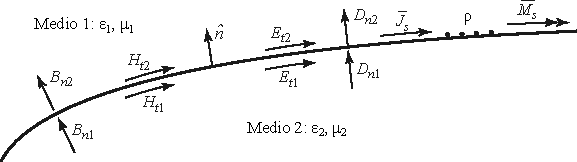
\includegraphics[width=0.8\textwidth]{intro_electro/condiciones_borde.pdf}
	\caption{Corrientes, campos y carga superficial en una interfaz general entre dos medios \cite{Pozar:MwEngineering}.}.
	\label{fig:condiciones_borde}
\end{figure}

Si se considera una interfaz entre dos medios, como la que se muestra en la figura \ref{fig:condiciones_borde}, a partir de las ecuaciones de Maxwell y los teoremas integrales, se pueden deducir las siguientes condiciones de borde:
\begin{subequations}
	\label{eq:condiciones_borde}
	\begin{align}
		\hat{n} \cdot (\vec{D}_{2} - \vec{D}_{1}) & = \rho_s \\
		\hat{n} \cdot (\vec{B}_{2} - \vec{B}_{2}) & = 0 \\
		\hat{n} \times (\vec{E}_2 - \vec{E}_1)  & = - \vec{M}_s \\
		\hat{n} \times (\vec{H}_2 - \vec{H}_1) & = \vec{J}_s
	\end{align}
\end{subequations}

\subsubsection{Campos sobre una superficie dieléctrica}
Dado que en una interfaz entre dos dieléctricos no hay carga eléctrica ni densidades de corriente, las ecuaciones \ref{eq:condiciones_borde} establecen que las componentes normales de los vectores $\vec{D}$ y $\vec{B}$ se conservan, y que las componentes tangenciales de $\vec{E}$ y $\vec{H}$ también lo hacen.

\subsubsection{Campos sobre una superficie conductora eléctrica}
Si el conductor no tiene pérdidas ($\sigma \rightarrow \infty$), todos los campos deben ser cero en su interior, dado que la profundidad de penetración se anula. Considerando, además, que $\vec{M}_s = 0$, la componente tangencial del campo eléctrico, $E_t$ desaparece sobre la superficie del conductor. Dado que la diferencia entre las componentes normales del campo magnético está dada por $\vec{J}_s$, y el campo magnético debe anularse en el conductor, la densidad de corriente superficial está dada únicamente por el campo magnético externo al conductor. En el mismo sentido, la densidad de carga superficial $\rho_s$ es la expresión, sobre la superficie del conductor, de la componente normal de $\vec{D}$.

% SKIN DEPTH

\subsubsection{Campos sobre una superficie conductora magnética}
Dado que la superficie conductora magnética representa el caso dual al de la superficie conductora eléctrica, en este caso se espera que la componente tangencial de $\vec{H}$ se anule sobre la superficie, mientras que la componente tangencial del campo eléctrico dé lugar a corrientes magnéticas sobre la misma.

%%%%% QUEDA DECRI QUE PASA CON UNA CORRIWENTE EN HORIZRAON O VERTICAL - LIBRO DE YAMAT, PAG 10.
%% COMPLETAR CON COLLIN %%

\section{Ecuación de onda}
\label{subsec_eq_de_onda}
%%%%

Al considerar una región del espacio lineal, isotrópica y homogénea, se puede calcular el rotor de la primera ecuación de Maxwell y aplicar la segunda ecuación \footnote{Se deberá utilizar la identidad $\nabla \times \nabla \times \vec{E} = \nabla \nabla \cdot \vec{E} - \nabla^2\vec{E}$, donde $\nabla \cdot \vec{E} = \rho/\epsilon$.}:

\begin{align}
	\nabla \times \nabla \times \vec{E} & = -j \omega \mu \nabla \times \vec{H} - \nabla \times \vec{M} \notag \\
	\nabla \nabla \cdot \vec{E} - \nabla^2 \vec{E} & = -j \omega \mu \nabla \times \vec{H} - \nabla \times \vec{M} \notag \\
	\frac{\nabla \rho}{\epsilon} - \nabla^2 \vec{E} & = \omega^2 \mu \epsilon \vec{E} - j \omega \mu \vec{J} - \nabla \times \vec{M} \notag\\
	\nabla^2 \vec{E} + \omega^2 \mu \epsilon \vec{E} & = j \omega \mu \vec{J} + \frac{\nabla \rho}{\epsilon} + \nabla \times \vec{M}
	\label{eq:eq_ondas_completa_E}
\end{align}

en el mismo sentido, para el campo magnético:
\begin{align}
	\nabla \times \nabla \times \vec{H} & = j \omega \nabla \times \vec{D} +  \nabla \times \vec{J} \notag \\
	\nabla \nabla \cdot \vec{H} - \nabla^2 \vec{H} & = j \omega \epsilon \nabla \times \vec{E} + \nabla \times \vec{J} \notag \\
	\frac{1}{\mu} \nabla (\cancelto{0}{\nabla \cdot \vec{B}}) - \nabla^2 \vec{H} & = j \omega \epsilon (-j \omega \vec{B} - \vec{M}) + \nabla \times \vec{J} \notag \\
	\nabla^2 \vec{H} + \omega^2 \epsilon \mu \vec{H} & =  j \omega \epsilon \vec{M} - \nabla \times \vec{J}
	\label{eq:eq_ondas_completa_H}
\end{align}

De las ecuaciones anteriores se observa que el campo magnético está determinado por la componente rotacional de la corriente eléctrica, mientras que el campo eléctrico está determinado por todas las componentes de la misma. De manera análoga, se cumple la relación inversa para el caso de la corriente magnética.

Si, además, la región del espacio es libre de fuentes, se deducen las ecuaciones de Helmholtz para ambos campos, donde $k$ es la constante de propagación o número de onda, en unidades de $(1/m)$:

\begin{equation}
	\label{eq:Helmholtz}
	\begin{aligned}
		\nabla \times \vec{E} + k^2 \vec{E} &= 0  \\
		\nabla \times \vec{H} + k^2 \vec{H}& = 0 
	\end{aligned}
	\qquad \text{Helmholtz}
\end{equation}
%%%%

Para el caso sin pérdidas se puede expresar como $k = \omega \sqrt{\mu \epsilon}$, mientras que si se considera que existen pérdidas óhmicas,  su efecto puede ser considerado si  $k$ asume el valor complejo $-j\gamma$, donde:

\begin{align}
\label{eq:constante-propagacion-compleja}
\gamma = j\alpha + \beta &= j\omega \sqrt{\mu (\epsilon'-j\epsilon'') - j \sigma \epsilon/\omega} & \text{Cte. de propagación compleja}
\end{align}

Para el caso de un buen conductor:

\begin{align}
\gamma = j\alpha + \beta &= j \omega \sqrt{\mu \epsilon} \sqrt{\sigma/(\omega \epsilon)} = (1+j) \sqrt{\omega \mu \sigma/2} & \text{(buen conductor)}
\end{align}

lo que nos permite definir la profundidad de penetración como 

\begin{align}
\delta_s = 1/\alpha &= \sqrt{\frac{2}{\omega \mu \sigma}} & \text{Profundidad de penetración}
\end{align}

En coordenadas cartesianas, para resolver las ecuaciones \ref{eq:Helmholtz} resulta sencillo aplicar el método de separación de variables\footnote{En coordenadas cartesianas, $\nabla^2 E = \frac{\partial^2 \vec{E}}{\partial x^2} + \frac{\partial^2 \vec{E}}{\partial y^2} + \frac{\partial^2 \vec{E}}{\partial z^2}$. Reemplazando las coordenadas $E_i$ de $\vec{E}, i=x,y,z$ por funciones $f(x),g(y),h(z)$ independientes entre sí, se obtiene que $\frac{f''(x)}{f(x)} + \frac{g''(y)}{g(y)} + \frac{h''(z)}{h(z)} + k_0^2 = 0$. Como las funciones $f$,$g$ y $h$ son independientes, se deduce que $\frac{f''(x)}{f(x)} = -k_x^2$, $\frac{g''(y)}{g(y)} = -k_y^2$ y $\frac{h''(z)}{h(z)} = -k_z^2$.}, que da lugar a ecuaciones cuya solución es de la forma $e^{\pm j k_i i}$, con $i = x, y$ o $z$, respectivamente. Las soluciones con un signo positivo en el exponente corresponden a ondas que viajan en la dirección negativa ($-x, -y, -z$), mientras que las que tienen un signo negativo corresponden a ondas que viajan en la dirección positiva. Dado que ambas soluciones son válidas y posibles, en función de las condiciones de borde, en general la expresión de la propagación de los campos electromagnéticos quedará establecida como la suma de ambas, afectadas por un factor de amplitud dependiente de la coordenada evaluada.

Para el caso de ondas que viajan en la dirección positiva

\begin{equation}
	\label{eq:electric_field_wave_solution}
	\vec{E}(x,y,z) = \vec{E}_0 \;e^{-j(k_x x + k_y y + k_z z)} = \vec{E}_0 \;e^{-j\vec{k}\cdot\vec{r}}
\end{equation}

donde se consideró que $\vec{E}_0 = A \hat{x} + B \hat{y} + C \hat{z}$, $\vec{r} = x \hat{x} + y \hat{y} + z \hat{z}$ y

\begin{equation}
\label{eq:numero_de_onda}
k_x^2 + k_y^2 + k_z^2 = k_0^2 \\
\end{equation}


Al expresar la divergencia del campo eléctrico de la ecuación \ref{eq:electric_field_wave_solution}, se obtiene\footnote{Aplicando $\nabla \cdot (f \vec{A}) = \vec{A} \cdot \nabla f + f \nabla \cdot \vec{A}$ a la expresión, resulta $\nabla \cdot \vec{E} = \vec{E}_0 \cdot \nabla e^{-j \vec{k} \vec{r}} + e^{-j \vec{k} \vec{r}}\nabla \cdot \vec{E}_0$, donde $\nabla \cdot \vec{E}_0 =0$}:


\begin{align}
\nabla \cdot \vec{E} = \nabla \cdot \vec{E}_0 e^{-j\vec{k} \cdot \vec{r}} & = -j \vec{k} \cdot \vec{E}_0 e^{-j \vec{k} \cdot \vec{r}} = 0
\end{align}

De lo que se puede deducir que $\vec{k} \cdot \vec{E}_0 = 0$, de modo que el campo eléctrico, en una onda plana, es siempre perpendicular a la dirección de propagación.

De la ecuación de Faraday de \ref{eq:Maxwell}, considerando espacio libre de cargas, se puede deducir que, para una onda plana, el campo magnético es siempre ortogonal al campo eléctrico y a la dirección de propagación, y que los campos están relacionados de forma que \cite{Fernandez:Electromag}:

\begin{align}
	\label{eq:relacion-e-h-ondaplana}
	\vec{H}(\vec{r},t) &= \pm \frac{\hat{n} \times \vec{E}(\vec{r},t)}{\eta}  & \text{Relación E y H en onda plana}
\end{align}

donde $\eta$ es la impedancia de onda, que tiene la forma

\begin{align}
	\eta &= \frac{j \omega \mu}{\gamma }& \text{Impedancia de onda}
\end{align}

Para el caso con pérdidas, y considerando que la dirección de propagación es $z$, las componentes $x$ e $y$ se comportan como:

\begin{equation}
E_i(z) = E_i \; e^{-\gamma z} = E_i \; e^{-\alpha z} \; e^{-j \beta z}, \quad i=x,y \nonumber
\end{equation}

En el caso del vacío, la impedancia intrínseca se denota $\eta_0$ y tiene un valor de $377\; \Omega$, mientras que para otros materiales está determinada por su permitividad eléctrica y permeabilidad magnética, y puede ser compleja si hay pérdidas.

La velocidad de fase se define como $v_p=\omega/\beta$, que para el caso sin pérdidas queda como $1/\sqrt{\mu \epsilon}$, y que para el caso particular del vacío, se expresa como $1/\sqrt{\mu_0 \epsilon_0} = c$, donde $c$ es la velocidad de la luz en el vacío. Así, la velocidad de fase en cualquier medio material sin pérdidas resulta $c/\sqrt{\epsilon_r \mu_r}$.

La longitud de onda, $\lambda$, es la distancia espacial entre dos máximos sucesivos, por lo que se expresa como $\lambda = 2\pi / k = v_p/f$.

\subsection{Incidencia de una onda plana sobre una interfaz}

Una onda electromagnética incidente sobre una superficie en un ángulo arbitrario puede analizarse descomponiendo el problema en dos casos canónicos de polarización (dirección del campo eléctrico): perpendicular (TE, transversal eléctrico) o paralela (TM, transversal magnético) al plano de incidencia, que es el formado por el rayo incidente y la normal a la interfaz. El problema de la incidencia perpendicular a la interfaz combina ambos casos.

\begin{figure} [H]
	\centering 
	\subfigure[Polarización paralela (TM).]{
		\label{fig:oblique_incidence_parallel}
		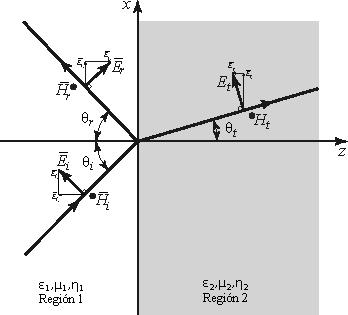
\includegraphics[width=0.45\textwidth]{intro_electro/incidencia_oblicua_paralela-version2.pdf}}
	\hspace{5mm}
	\subfigure[Polarización perpendicular (TE).]{
		\label{fig:oblique_incidence_perp}
		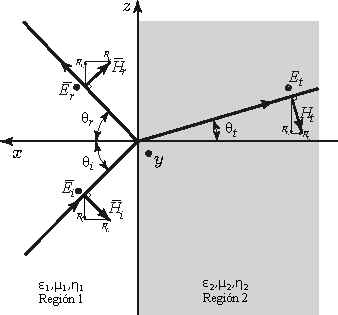
\includegraphics[width=0.45\textwidth]{intro_electro/incidencia_oblicua_perpendicular-version2.pdf}}
	\caption{Incidencia oblicua para los dos casos de polarización analizados.}
	\label{fig:oblique_incidence}
\end{figure}

Los campos eléctrico y magnético incidentes, según el sistema de coordenadas definido en la figura \ref{fig:oblique_incidence}, pueden ser expresados, en forma general, usando las expresiones \ref{eq:electric_field_wave_solution} y \ref{eq:relacion-e-h-ondaplana}, y considerando que no hay pérdidas, como indican las ecuaciones \ref{eq:incident_fields}:

\begin{align}
	\label{eq:incident_fields}
	\vec{E}_i &= \vec{E}_0 \;e^{-j\vec{k}_1 \cdot \vec{r}} &
	\vec{H}_i = \frac{\hat{k}_1 \times \vec{E}_0}{\eta_1} \;e^{-j\vec{k}_1 \cdot \vec{r}}
\end{align}

donde $\vec{r}=(x,y,z)$, $\vec{k}_1 = \hat{k}_1 \;\omega \sqrt{\mu_1 \epsilon_1}$, $\hat{k}_1$ es la dirección de propagación de la onda plana, y $\eta_1 = \sqrt{\mu_1 / \epsilon_1} = j\omega \mu / \gamma$ es la impedancia de onda de región de incidencia.

Se define al coeficiente de reflexión $\Gamma$ como la relación entre la magnitud del campo reflejado y del campo incidente, $E_r / E_i$. De la misma manera, el coeficiente de transmisión $T$ es la relación entre el módulo del campo transmitido al segundo medio y el campo incidente desde el primer medio, $E_t / E_i$, de manera que $1+\Gamma = T$ y que $(1-\Gamma)/\eta_1 = T/\eta_2$. 

Usando estos coeficientes, a partir de las ecuaciones \ref{eq:incident_fields}, y teniendo en cuenta las condiciones de borde descriptas en la sección \ref{sec:condiciones-borde}, se pueden calcular los campos reflejados y transmitidos. Para los dos casos canónicos analizados, los campos incidentes, reflejados y transmitidos se resumen en la tabla \ref{table:incidencia_oblicua}, así como los coeficientes de reflexión y transmisión.

\tabulinesep=1.2mm
\taburulecolor{black!20}
\begin{table}
	
	\begin{tabu} to 1\textwidth {gX[c]@{}X[c]@{}}
		\rowcolor{black!20} & \multicolumn{1}{c}{\textbf{TM}} & \multicolumn{1}{c}{\textbf{TE}}\\
		$\vec{E}_i$
		&
		\scalebox{0.86}{%
			$
			E_0\; (\hat{z}\; \mathrm{cos}\; \theta_i + \hat{x}\; \mathrm{sin}\; \theta_i)\; e^{-j k_1 (z\; \mathrm{sin}\; \theta_i - x\; \mathrm{cos}\; \theta_i)}
			$
		}	
		&
		\scalebox{0.86}{%
			$
			E_0\; \hat{y} \;e^{-j k_1 (z\; \mathrm{sin}\; \theta_i - x\; \mathrm{cos}\; \theta_i)}
			$
		} \\
		$\vec{H}_i$
		&
		\scalebox{0.86}{%
			$
			\frac{E_0}{\eta_1}\; \hat{y}\; e^{-j k_1 (z\; \mathrm{sin}\; \theta_i - x\; \mathrm{cos}\; \theta_i)}
			$
		}
		&
		\scalebox{0.86}{%
			$
			\frac{E_0}{\eta_1} \;(-\hat{z}\; \mathrm{cos}\; \theta_i - \hat{x}\; \mathrm{sin}\; \theta_i)\; e^{-j k_1 (z\; \mathrm{sin}\; \theta_i - x\; \mathrm{cos}\; \theta_i)}
			$
		} \\
		\hline
	
		$\vec{E}_r$
		&
		\scalebox{0.86}{%
			$
			E_0\; \Gamma\; (\hat{z}\; \mathrm{cos}\; \theta_r - \hat{x}\; \mathrm{cos}\; \theta_r)\; e^{-j k_1 (x\; \mathrm{sin}\; \theta_r + z\; \mathrm{sin}\; \theta_r)}
			$
		}	
		&
		\scalebox{0.86}{%
			$
			E_0\; \Gamma\; \hat{y} \;e^{-j k_1 (z\; \mathrm{sin}\; \theta_r + x\; \mathrm{cos}\; \theta_r)}
			$
		} \\
		$\vec{H}_r$
		&
		\scalebox{0.86}{%
			$
			-\frac{E_0\; \Gamma}{\eta_1}\; \hat{y}\; e^{-j k_1 (x\; \mathrm{sin}\; \theta_r + z\; \mathrm{sin}\; \theta_r)}
			$
		}
		&
		\scalebox{0.86}{%
			$
	 		\frac{E_0\; \Gamma}{\eta_1} \;(\hat{z}\; \mathrm{cos}\; \theta_r - \hat{x}\; \mathrm{sin}\; \theta_r)\; e^{-j k_1 (z\; \mathrm{sin}\; \theta_r + x\; \mathrm{cos}\; \theta_r)}
			$
		} \\
	\hline
		$\vec{E}_t$
		&
		\scalebox{0.86}{%
			$
			E_0\; T\; (\hat{z}\; \mathrm{cos}\; \theta_t + \hat{x}\; \mathrm{sin}\; \theta_t) e^{-j k_2 (z\; \mathrm{sin}\; \theta_t - x\; \mathrm{cos}\; \theta_t)}
			$
		}
		&
		\scalebox{0.86}{%
			$
			E_0\; T\; \hat{y}\; e^{-j k_2 (z\; \mathrm{sin}\; \theta_t - x\; \mathrm{cos}\; \theta_t)}
			$
		} \\
		$\vec{H}_t$
		&
		\scalebox{0.86}{%
			$
	 		\frac{E_0\; T}{\eta_1}\; \hat{y}\; e^{-j k_2 (z\; \mathrm{sin}\; \theta_t - x\; \mathrm{cos}\; \theta_t)}
			$
		}
		&
		\scalebox{0.86}{%
			$
			\frac{E_0\; T}{\eta_2}\; (-\hat{z}\; \mathrm{cos}\; \theta_t - \hat{x}\; \mathrm{sin}\; \theta_t)\; e^{-j k_2 (z\; \mathrm{sin}\; \theta_t - x\; \mathrm{cos}\; \theta_t)}
			$
		} \\
		\hline
		
		$\Gamma$
		&
		$\frac{\eta_2\; \cos\; \theta_t - \eta_1 \; \cos\; \theta_i}{\eta_2\; \cos\; \theta_t + \eta_1 \; \cos\; \theta_i}$
		&
		$\frac{\eta_2\; \cos\; \theta_i - \eta_1 \; \cos\; \theta_t}{\eta_2\; \cos\; \theta_i + \eta_1 \; \cos\; \theta_t}$
		\\
		$T$
		&
		$\frac{2 \;\eta_2 \; \cos\; \theta_i}{\eta_2\; \cos\; \theta_t + \eta_1 \; \cos\; \theta_i}$
		&
		$\frac{2\; \eta_2 \; \cos\; \theta_i}{\eta_2\; \cos\; \theta_i + \eta_1 \; \cos\; \theta_t}$
	\end{tabu}
	\caption{Campos incidentes, transmitidos y reflejados, y coeficientes de reflexión y transmisión para incidencia oblicua de una onda plana sobre una interfaz dieléctrica.}
	\label{table:incidencia_oblicua}
\end{table}

Si se fuerza la continuidad de las componentes tangenciales de los campos sobre la interfaz para ambos casos, $\vec{E}_i^{tg} + \vec{E}_r^{tg} = \vec{E}_t^{tg}$ y $\vec{H}_i^{tg} + \vec{H}_r^{tg} = \vec{H}_t^{tg}$, se obtienen las expresiones \ref{eq:continuidad_campos_paralelo} para el modo TM, y \ref{eq:continuidad_campos_perpendicular} para el modo TE.

\begin{equation}
	\begin{aligned}
		cos \; \theta_i \; e^{-j k_1 z \sin \; \theta_i} + \Gamma \; cos \; \theta_r \; e^{-j k_1 z \; \sin\; \theta_r} &= T\; \cos\; \theta_t \; e^{-j k_2 z \; \sin\; \theta_t}\\
		\frac{1}{\eta_1} \; e^{-j k_1 z \; \sin \theta_i} - \frac{\Gamma}{\eta_1} \; e^{-j k_1 z \; \sin \; \theta_r} &= \frac{T}{\eta_2} \; e^{-j k_2 z \; \sin\; \theta_t}
	\end{aligned}
	\label{eq:continuidad_campos_paralelo}
\end{equation}

\begin{equation}
	\begin{aligned}
		e^{-j k_1 z \sin \; \theta_i} + \Gamma \; e^{-j k_1 z \; \sin\; \theta_r} &= T\; e^{-j k_2 z \; \sin\; \theta_t}\\
		-\frac{1}{\eta_1} \cos\; \theta_i \; e^{-j k_1 z \; \sin \theta_i} - \frac{\Gamma}{\eta_1} \; \cos\; \theta_r e^{-j k_1 z \; \sin \; \theta_r} &= -\frac{T}{\eta_2} \; \cos\; \theta_t \; e^{-j k_2 z \; \sin\; \theta_t}
	\end{aligned}
	\label{eq:continuidad_campos_perpendicular}
\end{equation}

En estas ecuaciones se observa que a ambos lados de las igualdades, las expresiones son funciones de la posición sobre la interfaz. Para que la condición de borde se cumpla en todos sus puntos, la variación en $z$ debe ser la misma en todos los términos, de forma que el efecto de la variación sea anulado: $k_1 \; \sin\; \theta_i = k_1 \; \sin \; \theta_r = k_2 \; \sin\; \theta_t$.  De esta consideración se deriva la Ley de Snell (asumiendo que $\mu_1 = \mu_2$), expresada en la ecuación \ref{eq:snell_law}. En la gráfica de la figura \ref{fig:ley_snell} se puede observar el comportamiento del ángulo de refracción según en ángulo de incidencia la incidencia sobre una interfaz entre aire y FR4, en sentidos opuestos.

\begin{subequations}
	\label{eq:snell_law}
	\begin{align}
	\theta_i &= \theta_r & \text{Snell para reflexión}\\
	k_1 \; \sin\; \theta_i = k_2 \; \sin\; \theta_t & \overset{\eta=\frac{\omega\mu}{k}}{\Longrightarrow} \eta_2 \; \sin\; \theta_i = \eta_1 \; \sin\; \theta_t & \text{Snell para refracción}\label{eq:snell_law_second}
	\end{align}
\end{subequations}

\begin{figure}[htp]
	\centering
	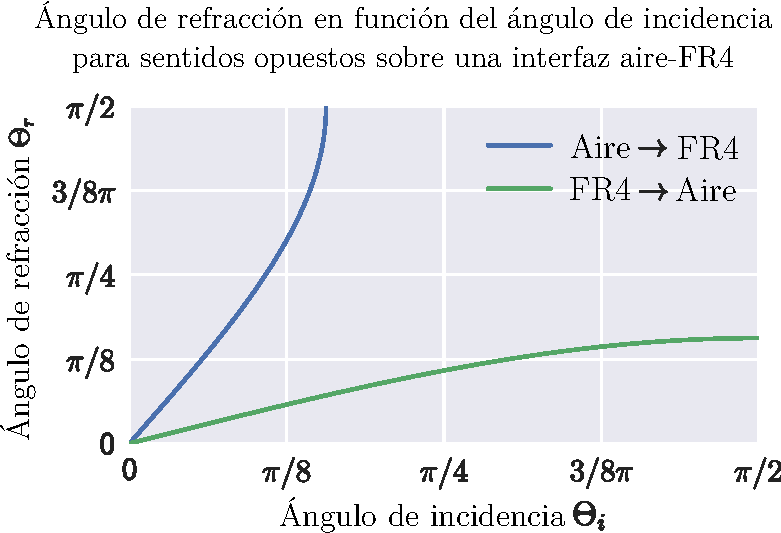
\includegraphics[width=0.7\textwidth]{intro_electro/angulo-refraccion-snell.pdf}
	\caption{Ángulo de refracción en función del ángulo de incidencia, según la ley de Snell.}
	\label{fig:ley_snell}
\end{figure}

Utilizando estas expresiones, y a partir de las ecuaciones \ref{eq:continuidad_campos_paralelo} y \ref{eq:continuidad_campos_perpendicular}, se obtienen las expresiones para los coeficientes de reflexión y transmisión de la tabla \ref{table:incidencia_oblicua}. Resulta importante destacar que, para el caso de incidencia perpendicular ($\theta_i = 0$), los coeficientes quedan simplificados a $\Gamma = (\eta_2 - \eta_1)/(\eta_2 + \eta_1)$ y $T = (2 \; \eta_2)/(\eta_2 + \eta_1)$.

Los coeficientes de transmisión y reflexión para incidencia oblicua, en ambas polarizaciones, se pueden graficar en función del ángulo incidente, teniendo en cuenta las ecuaciones de Snell para expresar el ángulo de transmisión en función del ángulo de incidencia. Estas gráficas se muestran, para la interfaz aire-FR4, en la figura \ref{fig:coeficientes-aire-fr4}, donde, además,  teniendo en cuenta la constante de propagación compleja de la ecuación \ref{eq:constante-propagacion-compleja}, se graficó también el caso con pérdidas, donde se observa, en general, una mayor reflexión y, por tanto, menor transmisión. Para ángulos de incidencia rasantes, la transmisión es mínima y la reflexión es máxima.

Resulta ilustrativo, además, graficar el comportamiento según el ángulo de incidencia de la misma interfaz, pero en el sentido dieléctrico-aire. Este gráfico se observa en la figura \ref{fig:coeficientes-fr4-aire}, donde los coeficientes de transmisión pueden ser mayores a 1 porque el ángulo de transmisión es menor al de incidencia, permitiendo conservar el flujo de energía por unidad de área.

\begin{figure}[H]
	\centering 
	\subfigure[Coeficiente de reflexión entre aire y FR4 en función de $\theta_i$.]{
		\label{fig:coeficiente-reflexion-aire-fr4}
		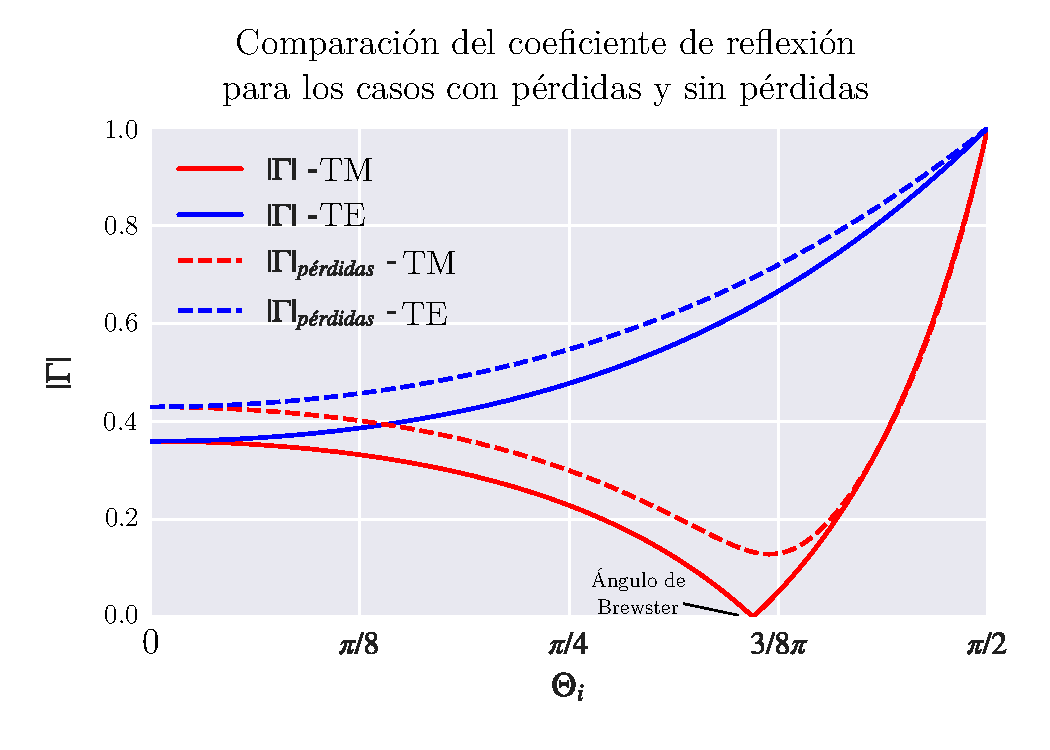
\includegraphics[width=0.48\textwidth]{intro_electro/plot-comparacion-lossy-lossless-annotated.pdf}}
	\subfigure[Coeficiente de transmisión entre aire y FR4 en función de $\theta_i$.]{
		\label{fig:coeficiente-transmision-aire-fr4}
		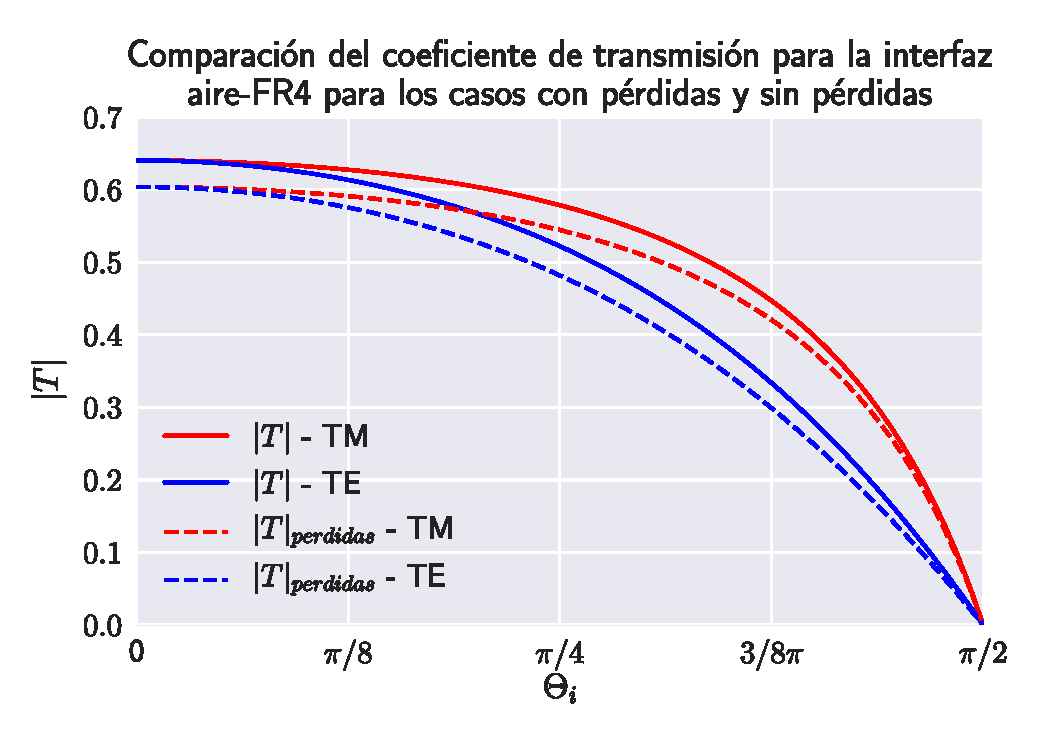
\includegraphics[width=0.48\textwidth]{intro_electro/plot-comparacion-lossy-lossless-T.pdf}}
	\caption{Coeficientes de transmisión y reflexión para el caso en que el medio de incidencia es aire, y el medio de transmisión es FR4.}
	\label{fig:coeficientes-aire-fr4}
\end{figure}


\begin{figure}[htp]
	\centering
	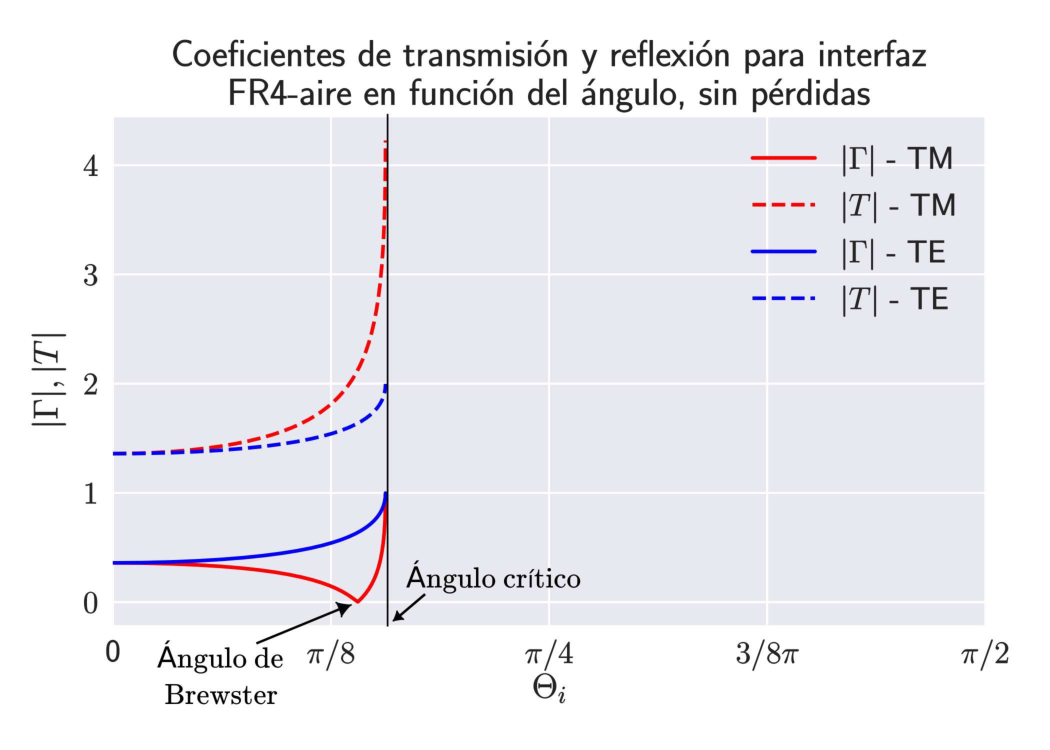
\includegraphics[width=0.7\textwidth]{intro_electro/plot-coeficientes-fresnel-dirInversa.pdf}
	\caption{Comportamiento de los coeficientes de reflexión y transmisión para el caso de incidencia FR4-aire.}
	\label{fig:coeficientes-fr4-aire}
\end{figure}



\subsection{Ángulo de Brewster y ángulo crítico}

Se conoce como ángulo de Brewster al ángulo de incidencia $\theta_i$ necesario para que se produzca reflexión nula ($\Gamma = 0$) en una interfaz, cuando sobre ella incide una onda plana en forma oblicua. Este efecto se da únicamente para la polarización TM, es decir, cuando existe componente de campo eléctrico en la dirección normal a la intefaz, por lo que suele ser utilizado como mecanismo para lograr polarización de una onda electromagnética.

Si se anulan los coeficientes de reflexión mostrados en la tabla \ref{table:incidencia_oblicua}, y se utilizan las ecuaciones \ref{eq:snell_law}, se puede la polarización TE no presenta ángulo de Brewster\footnote{Para lograr reflexión nula en TE se requiere que $\sin \; \theta_i / \sin \; \theta_t = cos \; \theta_i / cos \; \theta_t = \eta_1 / \eta_2$, lo cual es imposible.}, aunque sí lo hace la polarización TM\footnote{Para lograr reflexión nula en TE se requiere que $\sin \; \theta_i / \sin \; \theta_t = cos \; \theta_t / cos \; \theta_i = \eta_1 / \eta_2$, lo cual no supone una contradicción. Multiplicando la ecuación \ref{eq:snell_law_second} y el valor de $\Gamma$ para polarización TM, se obtiene que $\sin\;\theta_i \; cos \; \theta_i = \sin \; \theta_t \; cos \; \theta_t$, ó $\sin \; 2\theta_i = \sin \; 2\theta_t$, que se satisface cuando $2\theta_i = \pi - 2\theta_t$, de modo que $\theta_i + \theta_t = \pi/2$.}, de forma que $\theta_i + \theta_t = \pi/2$. Aplicando esta condición en la Ley de Snell (ecuación \ref{eq:snell_law_second}) se obtiene la expresión del ángulo de Brewster:

%%% GRAFICAR LO DE ACA ARRIBA, REEMPLAZANDO THETA_T POR LA LEY DE SNELL. EJE X: THETA_I. DE ESTA MANERA SE PODRIA VERIFICAR QUE PARA TE NO HAY SOLUCION Y PARA TM SI.

\begin{align}
	\label{eq:Brewster_angle}
	\tan\;\theta_B &= \frac{\eta_1}{\eta_2} = \sqrt{\frac{\epsilon_2}{\epsilon_1}} & \text{Relación del ángulo de Brewster}
\end{align}

Como se observa en la figura \ref{fig:Brewster-funcion-epsilon}, el ángulo de Brewster tiende a $90^{\circ}$ cuando la permeabilidad eléctrica del segundo medio es mucho mayor a la del primero, lo que significa que para evitar reflexiones, el ángulo de incidencia debe ser rasante. Cuando se da el caso contrario, en que la permeabilidad eléctrica del medio incidente es mayor a la del medio de transmisión, el ángulo de Brewster se vuelve menor a $45^{\circ}$, de lo que se deduce que una incidencia \textit{casi} perpendicular a la interfaz, y en consecuencia con polarización \textit{cercana} a TEM (aunque no exactamente TEM) lograría evitar la reflexión. El ángulo de $45^{\circ}$ cuando las permeabilidades eléctricas de ambos medios son iguales es meramente anecdótico, ya que si no existen diferencias entre los dos medios que forman la interfaz, la misma no existe, y por lo tanto no hay onda reflejada para \textit{ningún} ángulo de incidencia.

\begin{figure} [H]
	\centering 
	\subfigure[Ángulo de Brewster en función de $\epsilon_2/\epsilon_1$.]{
		\label{fig:Brewster-funcion-epsilon}
		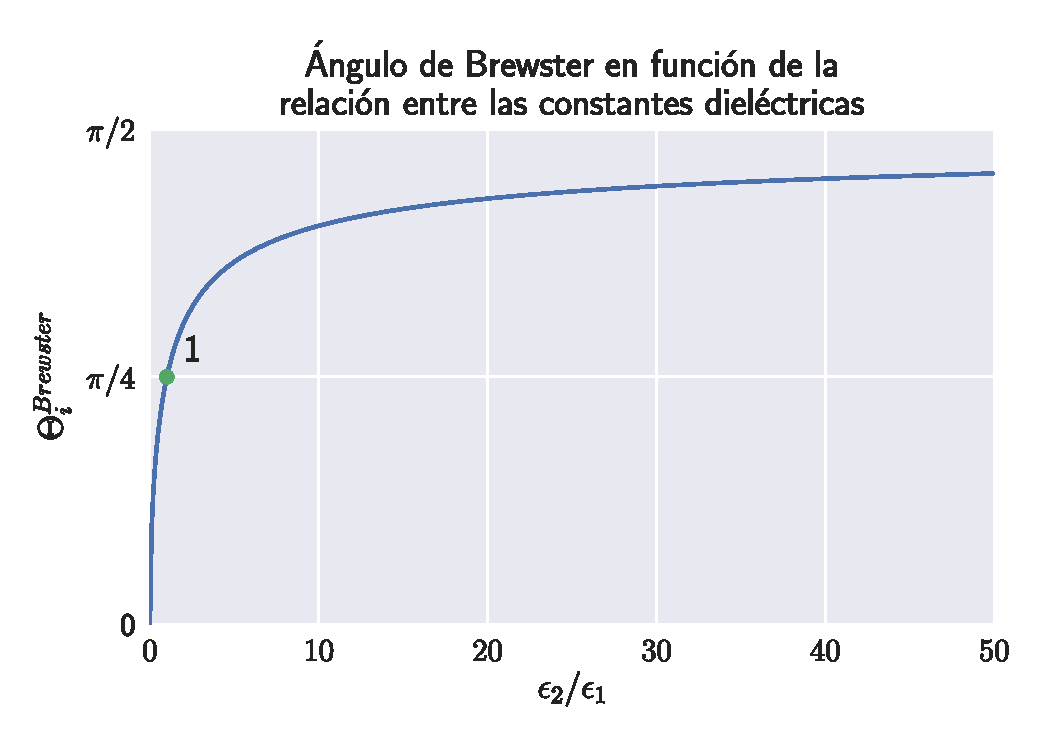
\includegraphics[width=0.48\textwidth]{intro_electro/plot-brewster.pdf}}
	\subfigure[Ángulo crítico y rango de reflexión total en función de $\epsilon_2/\epsilon_1$.]{
		\label{fig:angulo-critico-funcion-epsilon}
		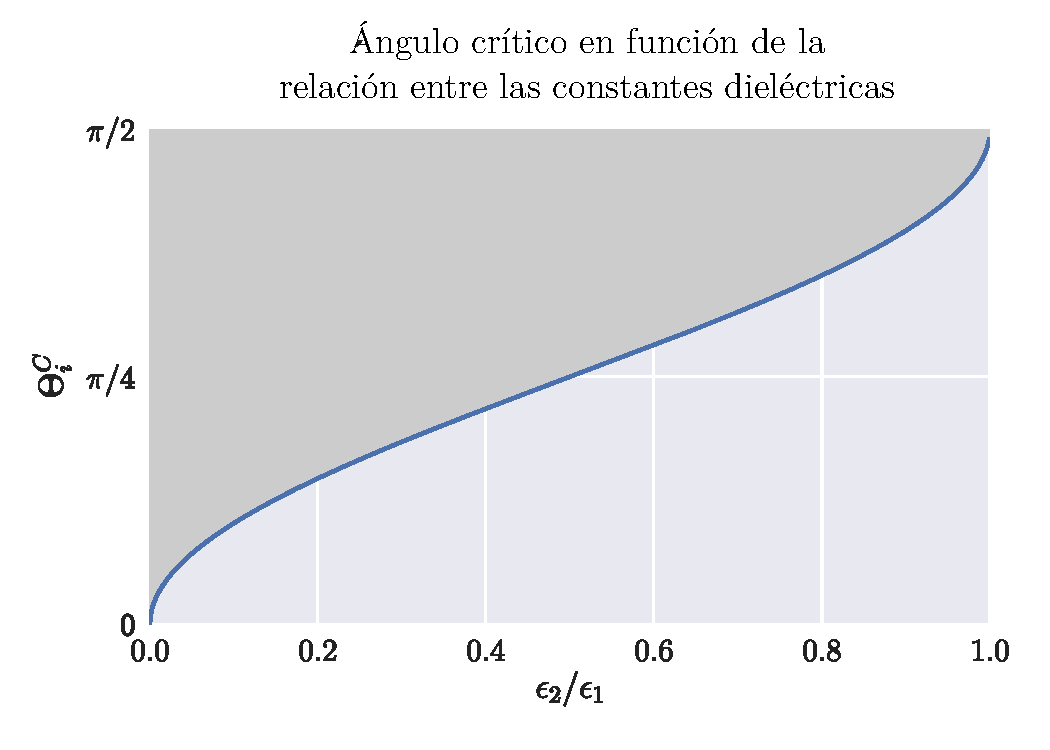
\includegraphics[width=0.48\textwidth]{intro_electro/plot-angulo-critico.pdf}}
	\caption{}
	\label{fig:angulo-critico-epsilon}
\end{figure}

En la figura  \ref{fig:coeficientes-aire-fr4} se puede observar el comportamiento de los coeficientes de reflexión y transmisión alrededor del ángulo de Brewster para polarización TM, cuando no se consideran pérdidas. Para polarizacón TE, el ángulo de Brewster no existe, y una situación similar se da cuando existen pérdidas en los materiales, incluso para polarización TM. En la figura \ref{fig:coeficientes-fr4-aire} también se puede observar el fenómeno de ángulo de Brewster, aunque debido a la dirección de la onda incidente, el mismo es mucho menor.


En ángulo crítico se define como el ángulo de incidencia para el cual la onda incidente es totalmente reflejada, y la onda transmitida no se propaga a la segunda región.

Si se observan las expresiones del coeficiente de transmisión de la tabla \ref{table:incidencia_oblicua}, el único valor de $\theta_i$ para el cual la transmisión es nula es $\pi/2$, es decir, incidencia rasante. Sin embargo, a partir de la ecuación \ref{eq:snell_law_second}, se obtiene que $\sin \; \theta_t = \eta_2 / \eta_1\; \sin\; \theta_i$. Se puede observar que en los casos en que $\eta_2 > \eta_1$ es posible que el ángulo de transmisión alcance el valor $\pi/2$ antes de que lo haga en ángulo de incidencia. El ángulo crítico, entonces, surge de la expresión \ref{eq:angulo_critico}, graficada en la figura \ref{fig:angulo-critico-epsilon}. En la gráfica se puede observar que si $\epsilon_2 = \epsilon_1$, el único ángulo para el que hay reflexión completa es el rasante. A medida que disminuye la relación entre las permeabilidades dieléctricas, el valor del ángulo crítico disminuye, hasta que el caso en que el valor de la permitividad dieléctrica del segundo medio es mucho mayor a la del primero, lo que vuelve a las impedancias de onda muy disímiles, generando que haya reflexión total para cualquier ángulo de incidencia.

\begin{equation}
	\label{eq:angulo_critico}
	\sin\; \theta_i^c = \frac{\eta_1}{\eta_2}\;\sin \; \theta_t|_{\theta_t=\pi/2} = \sqrt{\frac{\epsilon_2}{\epsilon_1}} \implies \theta_c = \arcsin \;\sqrt{\frac{\epsilon_2}{\epsilon_1}} = \arcsin \;\frac{\eta_1}{\eta_2}
\end{equation}

Para ángulos mayores a $\theta_c$, las expresiones del coeficiente de reflexión se vuelven complejas y de módulo 1, por lo que toda la energía electromagnética es reflejada, y la onda transmitida tiene un comportamiento evanescente, como se muestra en la figura \ref{fig:angulo_critico}. En la ecuación \ref{eq:angulo_critico} se observa que si $\theta_i > \theta_c$, el ángulo $\theta_t$ pierde significado físico, debido a que $\sin\; \theta_t$ debería ser mayor a 1 para cumplir la ecuación.

\begin{figure}[htp]
	\centering
	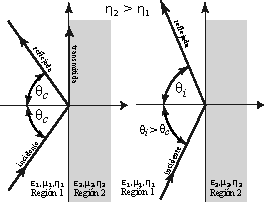
\includegraphics[width=0.6\textwidth]{intro_electro/angulo_critico.pdf}
	\caption{Ilustración del comportamiento de una onda plana durante la incidencia con ángulo critico y con ángulo mayor al $\theta_c$.}
	\label{fig:angulo_critico}
\end{figure}

Se debe notar que en el argumento anterior no se consideró la polarización de la onda incidente, por lo que la reflexión completa se puede dar tanto en modo TM como en modo TE, siempre y cuando la incidencia se produzca desde el medio ópticamente más denso al menos denso \cite{Fernandez:Electromag}, como se muestra en la figura \ref{fig:coeficientes-fr4-aire}. Sin embargo, resulta útil expresar el comportamiento de los campos.

Para el caso de una onda incidente con una polarización lineal arbitraria como la expresada en la ecuación \ref{eq:incident_fields}, se debe considerar que la componente longitudinal a la interfaz del vector de onda $\vec{k}$ se mantendrá constante, de modo que ${k_2}_x = {k_1}_x = k_1 \; \sin \; \theta_i$. La componente transversal a la interfaz, en cambio, será ${k_2}_z = k_2\; \cos \; \theta_t = k_2 \sqrt{1-sin^2\theta_t} = \beta$. Dado que para el caso en que el ángulo incidente es mayor al ángulo crítico se requiere que $\sin\;\theta_t > 1$, el valor de ${k_2}_z$ será imaginario, $-i\alpha$ \footnote{El signo negativo se desprende de la imposibilidad física de un crecimiento exponencial del valor del campo, lo cual descarga la posibilidad de que el signo sea positivo}. De esta forma, para direcciones de campos arbitrarias, y teniendo en cuenta el hecho de que el vector $\vec{k}$ se desarrolla sobre el plano de incidencia:

\begin{subequations}
	\begin{align}
		\vec{E}_t (\vec{r},t) = \vec{E}_2 \; e^{-j \vec{k}_2 \cdot \vec{r}} = \vec{E}_2 \; e^{-j({k_2}_x x + {k_2}_z z)} = \vec{E}_2 \; e^{-j(\beta x - j\alpha z)} = \vec{E}_2 \; e^{-j\beta x} \; e^{- \alpha z}\\
		\vec{H}_t (\vec{r},t) = \vec{H}_2 \; e^{-j \vec{k}_2 \cdot \vec{r}} = \vec{H}_2 \; e^{-j({k_2}_x x + {k_2}_z z)} = \vec{H}_2 \; e^{-j(\beta x - j\alpha z)} = \vec{H}_2 \; e^{-j\beta x} \; e^{- \alpha z}
	\end{align}
\end{subequations}

Se observa que en la dirección perpendicular a la interfaz hay un comportamiento evanescente o exponencial decreciente de la onda transmitida, mientras que existe propagación en la dirección paralela a la interfaz, dando lugar a lo que se conoce como onda de superficie.

La ecuación del módulo del vector de onda (\ref{eq:numero_de_onda}) resulta redefinida como $\beta^2 - \alpha^2 = k_2^2$, de donde se deduce que $\alpha = \sqrt{k_1^2\;sin^2\;\theta_i - k_2^2}$.



\section{Guias de ondas}
\label{subsec_guias_de_ondas}
%%%%
%Pozar, pag 171
%%%%

Suponiendo una guía de ondas de forma arbitraria en la que la energía electromagnética se propaga en la dirección $z$, los campos eléctrico y magnético se pueden expresar como la suma de sus componentes longitudinales (en la dirección $z$) y sus componentes transversales (en el plano $xy$), ambas con una constante de propagación $\gamma$ y dependientes sólo de la posición en el plano transversal, de manera que:

\begin{align}
	\vec{E}(x,y,z) = \left[ \vec{e}_{xy}(x,y) + \hat{z} e_z(x,y) \right] e^{-j\beta z}
\end{align}

Aplicando las ecuaciones rotacionales de Maxwell (Faraday y Ampère en la ecuación \ref{eq:Maxwell}), considerando una región libre de cargas y un comportamiento armónico de los campos, se puede deducir que las componentes transversales quedan en términos de las componentes longitudinales \cite{Fernandez:Electromag}:

\begin{equation}
	\begin{aligned}
		H_x &= \frac{j}{k_c^2} \left(\omega \epsilon \frac{\partial E_z}{\partial y} - \gamma \frac{\partial H_z}{\partial x} \right) & H_y &= \frac{-j}{k_c^2} \left(\omega \epsilon \frac{\partial E_z}{\partial x} + \gamma \frac{\partial H_z}{\partial y} \right)\\
		E_x &= \frac{-j}{k_c^2} \left(\omega \mu \frac{\partial H_z}{\partial y} + \gamma \frac{\partial H_z}{\partial x} \right) & E_y &= \frac{j}{k_c^2} \left(\omega \mu \frac{\partial H_z}{\partial x} - \gamma \frac{\partial E_z}{\partial y} \right)
	\end{aligned}
	\label{eq:campos_guia_de_ondas}
\end{equation}

donde se definió $k_c^2 = k^2 - \beta^2$ como el número de onda de corte, siendo $k = \omega \sqrt{\mu \epsilon} = 2\pi/\lambda$ el número de onda  en el material que rellena la línea de transmisión.

Cuando no existen componentes de campo en la dirección de propagación, $z$, según las ecuaciones \ref{eq:campos_guia_de_ondas}, no existen campos en las direcciones transversales si $k_c \neq 0$. La indeterminación generada por el hecho de que $k_c$ se anula da como resultado que $\beta = \omega \sqrt{\mu \epsilon} = k$, de modo que no existe número de onda de corte, y haciendo que la impedancia de onda sea $\eta$.  A este modo de propagación sobre una guía de ondas se lo llama TEM (transversal electromagnético). Los campos transversales satisfacen que el Laplaciano es 0, de modo que se comportan como un campo electrostático, y este es el motivo por el cual no pueden existir ondas TEM en guías de ondas de un único conductor.

Cuando la componente $z$ del campo eléctrico se anula, el modo de propagación se denomina TE (transversal electrico), y pueden utilizarse las relaciones descriptas en la ecuación \ref{eq:campos_guia_de_ondas} para obtener el resto de los campos. La impedancia de onda, en este caso, resulta $Z_{TE} = k\eta/\beta$, dependiente de la frecuencia.

Cuando la componente $z$ del campo magnético se anula, el modo de propagación es TM (transversal magnético), y con el mismo procedimiento que antes, se puede hallar su impedancia de onda, que resulta $Z_{TM} = \beta \eta / k$.

\subsection{Guía de ondas dieléctricas con plano de tierra}

\section{Ondas de superficie}

Existen estructuras abiertas que son capaces de mantener el campo electromagnético íntimamente ligadas a ellas, de forma que el mismo decaiga exponencialmente con la distancia a las mismas (comportamiento evanescente), y simultáneamente permiten propagación de energía en una dirección $z$ (con un decrecimiento inverso a la raiz cuadrada de la distancia, debido a la expansión del frente de onda), dando lugar a lo que se conoce como ondas de superficie \cite{Barlow:SurfaceWaves}. Estas estructuras se denominan guías de ondas superficiales, y pueden consistir en planos conductores recubiertos de dieléctrico, en planos corrugados o en simples interfaces entre dos medios distintos. Uller inauguró el campo en 1903, y luego Zenneck y Sommerfeld, entre 1907 y 1909, las utilizaron para explicar la propagación de ondas en la superficie terrestre, aunque este último utilizó la expresión ``ondas de superficie" para referirse al efecto conjunto de ondas espaciales y ondas de superficie \cite{Barlow:SurfaceWaves}, que no se corresponde con completamente con la definición actual. Recién en la década de 1950 se realizaron estudios teóricos de importancia, que permitieron hallar aplicaciones y nuevas estructuras que permiten la propagación de este tipo de ondas.

En la actualidad existen numerosos tipos de ondas de superficie, entre las que se destacan las ondas Zenneck (utilizadas en bajas frecuencias, cuando los medios intervinientes poseen altas pérdidas), las ondas de tipo resonante (que surgen cuando una onda incide sobre un material periódico), las ondas de superficie no lineales (que se generan en medios no lineales), los plasmones (utilizados en altas frecuencias, cuando los medios tienen bajas pérdidas) y las ondas de Dyakonov (donde al menos uno de los materiales es anisotrópico).

Para este trabajo, resultan de importancia las ondas de Zenneck, ya que permiten explicar el comportamiento de las ondas sobre una placa dieléctrica fina que posee un plano conductor en una de sus caras. Una representación tridimensional de las mismas se puede observar en la figura \ref{fig:onda-superficie-3d}.

\begin{figure}[htp]
	\centering
	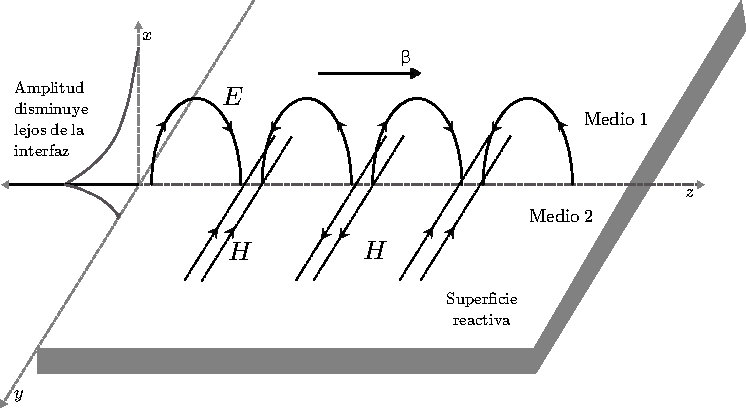
\includegraphics[width=0.8\textwidth]{intro_electro/ondas-superficie-3d.pdf}
	%\input{Figures/intro_electro/onda-superficie-incidencia-brewster3.pdf_tex}
	\caption{Representación gráfica del comportamiento de una onda de superficie sobre una interfaz reactiva.}
	\label{fig:onda-superficie-3d}
\end{figure}

Si se considera que una onda plana incide con ángulo de Brewster en modo TM sobre una interfaz entre dos medios de bajas pérdidas ($\epsilon'' \ll \epsilon'$), cada uno con una permitividad eléctrica $\epsilon_i$ y una permeabilidad magnética $\mu_i$, $i=1,2$, como indica la figura \ref{fig:onda-superficie-brewster}, no existirá energía reflejada. De esta forma, toda la energía incidente es entregada a la interfaz, y se obtienen las expresiones \ref{eq:ondas-superficie-campos}. Con el fin de simplificar dichas ecuaciones, se considera que el medio 1 es aire, de modo que $\epsilon_1 = \epsilon_0$, $\mu_1 = \mu_0$ y, en consecuencia, $\eta_1 = \eta_0$.

\begin{figure}[htp]
	\centering
	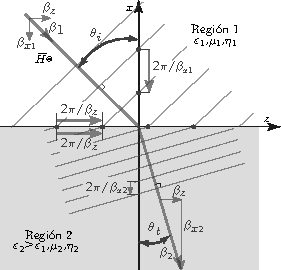
\includegraphics[width=0.5\textwidth]{intro_electro/onda-superficie-incidencia-brewster.pdf}
	%\input{Figures/intro_electro/onda-superficie-incidencia-brewster3.pdf_tex}
	\caption{Ilustración del comportamiento de una onda plana durante la incidencia con ángulo de Brewster. Las rectas paralelas representan los frentes de onda, es decir, son rectas de fase constante. Es importante destacar que la longitud de onda paralela a la interfaz, $2\pi/\beta$, se mantiene constante a ambos lados, dado que sobre la interfaz se intersectan las rectas de fase constante.}
	\label{fig:onda-superficie-brewster}
\end{figure}

\begin{subequations}
	\label{eq:ondas-superficie-campos}
	\begin{align}
	{H_1}_y &= A e^{-j\ (z\; \overbrace{k_0\;\sin \theta_i}^{\beta} - x\; \overbrace{k_0\;\cos \theta_i}^{h_1}}),\;\; x>0 & j\omega\epsilon E_x &= -\frac{\partial H_y}{\partial z} \\
	{H_2}_y &= A T e^{-j\; (z\; \overbrace{k\; \sin \theta_t}^{\beta} - x\; \overbrace{k\; \cos \theta_t)}^{h_2}},\;\; x<0   & j\omega\epsilon E_z &= -\frac{\partial H_y}{\partial x} 
	\end{align}
\end{subequations}

La componente longitudinal de los vectores de onda, $\beta$, es igual a ambos lados de la interfaz, como se muestra en la figura \ref{fig:onda-superficie-brewster}, de modo que es $k \; \sin \; \theta_t = \beta = k_0 \; \sin \; \theta_i$. Las componentes normales a la interfaz, que llamaremos $h_i$, $i=1,2$, deben cumplir la expresión de la ecuación \ref{eq:condicion-componentes-normales-ondas-superficie}, y están también mostradas en la figura \ref{fig:onda-superficie-brewster}.

\begin{align}
	\label{eq:condicion-componentes-normales-ondas-superficie}
	& h_1^2 + \beta^2 = k_0^2 &h_2^2 + \beta^2 = k^2
\end{align}

Las impedancias de onda en ambas regiones se obtienen como la relación entre los campos tangenciales a la interfaz sobre la que se incide, de modo que:

\begin{subequations}
\label{eq:impedancia-onda-superficie}
\begin{align}
	Z_1 = \frac{{E_z}_1}{{H_y}_1} = \eta_0 \; \cos\; \theta_i &\implies Z_1 = \frac{h_1}{k_0} \eta_0 \label{eq:impedancia-onda-incidente-onda-sup}\\
	Z_2 = \frac{{E_z}_2}{{H_y}_2} = \eta \; \cos \; \theta_t &\implies Z_2 = \frac{h_2}{k} \eta \label{eq:impedancia-onda-transmitida-onda-sup}
\end{align}
\end{subequations}

Para poder considerar que toda la energía de la onda incidente se transmite a la interfaz, debe suceder que las impedancias de onda a ambos lados de la interfaz sean iguales, de modo que $Z_1 = Z_2$. Igualando las ecuaciones \ref{eq:impedancia-onda-incidente-onda-sup} y \ref{eq:impedancia-onda-transmitida-onda-sup}, se deduce\footnote{Al igualar las expresiones de las impedancias de onda, se obtiene $\frac{h_1 \eta_0}{k_0} = \frac{h_2 \eta_2}{k}$. Recordando que $k_0=\omega \sqrt{\mu_0 \epsilon_0}$, $k=\omega \sqrt{\mu_0 (\epsilon'-j\epsilon'')}$, $\eta_0 = \sqrt{\mu_0 / \epsilon_0}$ y $\eta = \sqrt{\mu_0 / (\epsilon'-j\epsilon'')}$, se deduce que la relación entre $h_1$ y $h_2$ es compleja: $h_1\; (\epsilon' - j \epsilon'') = h_2 \epsilon_0$, de modo que en forma general se puede considerar que tanto $h_1$ como $h_2$ son complejos.} que, en forma general, si el medio sobre el que se incide tiene pérdidas, entonces $h_1$ y $h_2$ son complejos. De esta manera, $h_1 = h_1' - jh_1''$ y $h_2 = h_2' + jh_2''$, lo que significa que además de avanzar en fase, la onda pierde energía, pues tiene un comportamiento evanescente, de modo que el vector de Poynting tiene una componente en la dirección perpendicular a la interfaz, debido al consumo de energía de la misma \cite{Barlow:SurfaceWaves}. A mayores pérdidas, mayor será la inclinación del vector de Poynting resultante respecto de la interfaz. Como $\vec{k_0} = \vec{\beta} + \vec{h_1}$, la constante de propagación, $\beta = \beta' - j \beta''$, posee también un valor complejo.

El campo magnético queda determinado por:

\begin{equation}
	H_y =
	\left\lbrace
	\begin{aligned}
		A e^{-j\beta'z -\beta''z + (j h_1' - h_1'')x}, \quad x>0 \\
		A e^{-j\beta'z -\beta''z + (j h_2' + h_2'')x}, \quad x<0 \\
	\end{aligned}
	\right.
\end{equation}

Se observa que los planos de fase constante, en el aire, los correspondientes a las exponenciales imaginarias de la ecuación anterior, $\beta'z - h_1'x = cte$, y se muestran en la figura \ref{fig:onda-superficie-brewster}. Los planos de amplitud constante se obtienen considerando las exponenciales decrecientes de las expresiones, de forma que $\beta''z + h_1''x = cte$, que para el caso analizado en la figura \ref{fig:onda-superficie-brewster}, son rectas con pendiente negativa (no mostradas en la figura).

Para bajas pérdidas, $\beta''$ será pequeño, por lo que habrá baja atenuación para la onda que se desplaza en dirección $z$, pero debido a que $h_1''$ y/o $h_2''$ también serán bajas, la energía no estará concentrada cerca de la interfaz.



Si se considera una superficie con una impedancia de onda para polarización TM normalizada respecto de $\eta_0$, $Z_s = R_s + j X_s$, independiente del ángulo de incidencia, entonces, al igualar la impedancia de onda a la impedancia de superficie, y teniendo en cuenta las igualdades de la ecuación \ref{eq:impedancia-onda-superficie}, resulta:

\begin{align}
	h_1 & = k_0 \frac{Z_1}{\eta_0} = k_0 Z_s = k_0 R_s + j k_0 X_s \label{eq:h1-onda-superficie}\\
	\beta &= \beta' - j\beta'' =\sqrt{(k_0^2 - h_1^2)} = k_0 \sqrt{1+X_s^2 - R_s^2 - 2jR_s X_s} \label{eq:beta-onda-superficie}
\end{align}

La gráfica de las componentes real e imaginaria de $\beta$ se muestra en la figura \ref{fig:beta-reactancia-TM}. Se puede observar que, cuando la reactancia es inductiva (valores positivos de $X_s$), la parte imaginaria de $\beta$, $\beta''$, presenta valores positivos, por lo que habrá atenuación en la dirección de propagación $z$ ([a] en la figura) \footnote{Esto se debe a que si el campo eléctrico en la dirección $y$ se escribe como se indica en la ecuación \ref{eq:ondas-superficie-campos}, $\beta=\beta'-j\beta''$ y $h_1 = h_1'+jh_1''$, el exponente se expresa como $-j(\beta'-j\beta'')z + j(h_1'+jh_1'')x$. Para dirección de propagación $z$, con $z>0$, la componente de atenuación del exponente de la expresión dada resulta en $-\beta'' z$. Para que el comportamiento resulte decreciente, $\beta''$ debe ser mayor a $0$.}. A mayor reactancia, habrá una mayor disminución de la amplitud del campo a medida que aumenta el valor de $z$, aunque la mayor variación en el coeficiente de atenuación se observa con la variación de la resistencia, $R_s$, cuando existe un comportamiento reactivo apreciable ([b] en la figura).

Si la reactancia es nula, un valor de $\beta$ real se obtiene sólo si la resistencia es muy baja o nula ([c] en la figura). A partir de un umbral de resistencia de superficie, dependiente de los medios materiales, cuando no existe comportamiento reactivo, no hay propagación de onda de superficie ($\beta=0$, [d] en la figura).

El comportamiento de $h_1$, descripto en la ecuación \ref{eq:h1-onda-superficie} también regula el comportamiento de la onda de superficie, dado que si la parte imaginaria de $h_1$, $h_1''$, es muy pequeña, la onda no estará lo suficientemente cerca de la interfaz para ser guiada por ella. Un valor alto de $h_1''$ se da cuando la reactancia, $X_s$ es inductiva ($X_s>0$), lo cual coincide con el requisito para $\beta''$. Dicho de otra forma, la reactancia de superficie es la responsable del decrecimiento exponencial de la onda al aumentar la distancia con la interfaz que funciona como guía.

Analizando la ecuación \ref{eq:beta-onda-superficie}, se deduce que un producto $R_s X_s$ pequeño dará lugar a atenuaciones pequeñas en la onda de superficie, de modo que para que se propague una onda sobre la interfaz, si se establece $X_s$ grande para obtener un valor de $\beta'$ grande, se deben disminuir el comportamiento resistivo tanto como sea posible ([e] en la figura).

\begin{figure}[htp]
	\centering
	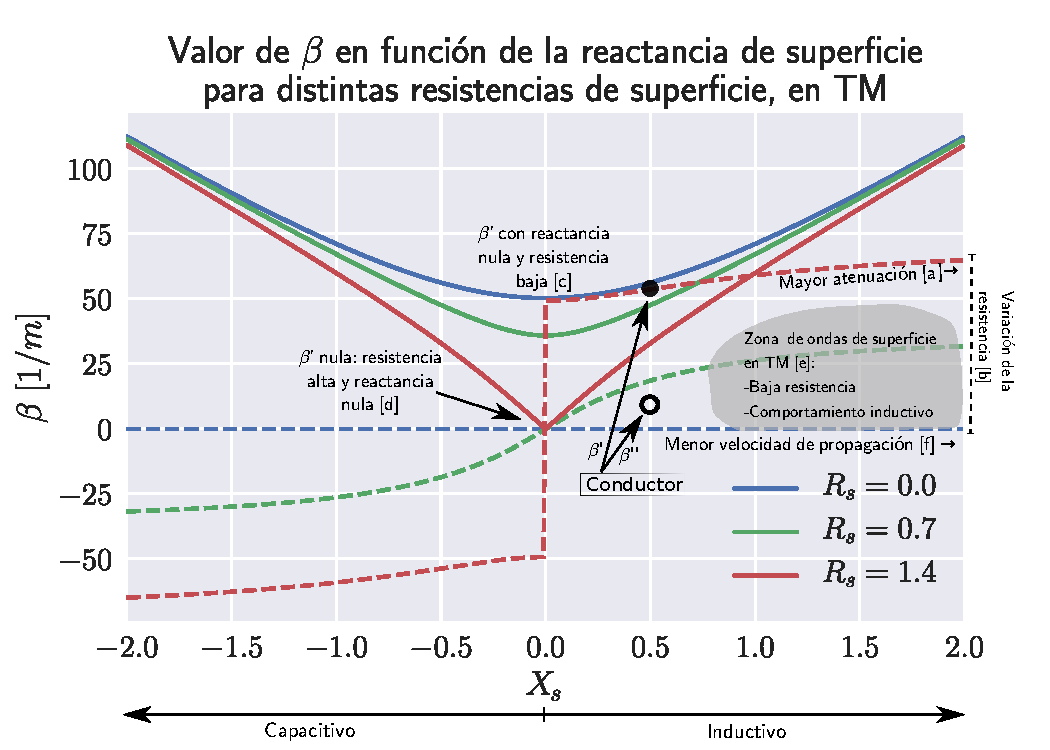
\includegraphics[width=\textwidth]{intro_electro/plot-beta-reactancia-TM.pdf}
	%\input{Figures/intro_electro/onda-superficie-incidencia-brewster3.pdf_tex}
	\caption{Comportamiento de la constante de propagación superficial $\beta$ en función de la resistencia y reactancia superficial para el caso de incidencia TM. Las líneas punteadas representan la parte imaginaria de $\beta$, y las líneas completas representan la parte real, de forma que $\beta = \beta' - j\beta''$.}
	\label{fig:beta-reactancia-TM}
\end{figure}

La velocidad de propagación se obtiene directamente de la componente real de $\beta$ que, si $R_s$ es pequeño y $X_s$ es grande, resulta, a partir de la expresión \ref{eq:beta-onda-superficie}, $\beta' = k_0 \sqrt{1+X_s^2}$, de forma que la velocidad de propagación es:

\begin{align}
	v_p = \frac{\omega}{\beta'} = \frac{c}{\sqrt{1+X_s^2}}
\end{align}

En los casos en que la componente reactiva de la impedancia de superficie es grande, el valor de la velocidad de propagación es menor al de la luz (denotado como [f] en la figura).

%%%%%%%%%%%%%%%%%

Cuando la interfaz es de tipo aire-conductor, la componente inductiva de la impedancia de superficie (relacionada a la profundidad de penetración) resulta igual a la componente resistiva, de forma que \cite{Fernandez:Electromag}:

\begin{align}
	\eta &= \frac{1+j}{\sigma \delta} &\text{Impedancia de superficie - conductor}
\end{align}
 
Aplicando las ecuaciones \ref{eq:impedancia-onda-superficie}, se obtiene que

\begin{align}
	h &= k_0 (1+j) \sqrt{\frac{k_0}{2 \sigma Z_0}} \\
	\beta &= k_0 \sqrt{1-\frac{j k_0}{\sigma Z_0}} \approx k_0 - \frac{j k_0^2}{2 \sigma Z_0}
\end{align}

En general, un plano conductor soporta ondas de superficie, y la atenuación en la dirección de propagación es muy baja (ver figura \ref{fig:beta-reactancia-TM}), pero no es capaz de lograr una atenuación en la dirección normal al mismo tal que la energía se mantenga concentrada en la superficie para poder ser utilizada como guía de ondas. Esto se debe a que dado que la parte imaginaria de $h_1$ también es despreciable, especialmente debido a la alta conductividad del metal. Para lograr que la energía de la onda decaiga rápidamente lejos de la interfaz es necesario aumentar considerablemente la reactancia de la superficie, para lo que se suele agregar al conductor una capa dieléctrica, que además no aumenta considerablemente la resistividad.

Para el caso de ondas de superficie en modo TE, los campos están dados por la ecuación \ref{eq:campo-electrico-superficie-TE}. La impedancia de onda, en tanto, queda expresada como indica la ecuación \ref{eq:impedancia-onda-superficie-TE}. Considerando que, para evitar reflexiones, la impedancia de superficie tiene que ser igual a la impedancia de onda, se obtiene la expresión para la constante de propagación en el sentido perpendicular a la interfaz mostrada en la ecuación \ref{eq:h1-onda-superficie-TE}, donde nuevamente la impedancia de superficie del conductor es $Z_s = R_s +jX_s$.

\begin{equation}
	\label{eq:campo-electrico-superficie-TE}
	\begin{aligned}
		E_y = A e^{jhx-j\beta z} \qquad j\omega \mu_0 H_z = -\frac{\partial E_y}{\partial x} \qquad j\omega \mu_0 H_x = \frac{\partial E_y}{\partial z}
	\end{aligned}
\end{equation}

\begin{align}
	\label{eq:impedancia-onda-superficie-TE}
	Z_1 = \frac{E_y}{H_z} = -\frac{\omega \mu_0}{h} = -\frac{\eta k_0}{h}
\end{align}

\begin{align}
	\label{eq:h1-onda-superficie-TE}
	h = -\frac{k}{Z_s} = -k_0 \frac{R_s}{{R_s^2 + X_s^2}}-j\frac{X_s}{R_s^2 + X_s^2}
\end{align}

Se observa que para que el valor de $h''$ resulte positivo, de manera que se de un decrecimiento exponencial desde la superficie, el valor de $X_s$ tiene que ser negativo, por lo que el comportamiento de la superficie tiene que ser capacitivo.

La segunda condición para la existencia de ondas de superficie, la propagación de los campos, está asegurada si $\beta'$ es positivo, y si la atenuación en la dirección de propagación, parametrizada por $\beta''$, es baja. La expresión de $\beta$ para el caso TE resulta, a partir de \ref{eq:h1-onda-superficie-TE}:

\begin{align}
	\beta = \beta'-j\beta''= \sqrt{(k_0^2 - h_1^2)} = \frac{k_0}{R_s^2+X_s^2} \sqrt{1+X_s^2 - R_s^2 + 2jR_s X_s} \label{eq:beta-onda-superficie-TE}
\end{align}

Gráficas de la expresión anterior se muestran en la figura \ref{fig:beta-reactancia-TE}, donde se pueden observar valores de $\beta'$ y $\beta''$ en función de la reactancia $X_s$, para algunos valores de resistencia de superficie $R_s$. Resulta importante destacar que para valores en que $X_s$ es negativa (reactancia capacitiva), el valor de $\beta''$ es físicamente realizable, ya que da lugar a un decrecimiento exponencial, y no a un incremento. Por otro lado, al contrario que en el caso de las ondas TM, a medida que la reactancia capacitiva aumenta en módulo, la constante de propagación tiende a estabilizarse en lugar de crecer linealmente, aunque sí decrece la constante de atenuación $\beta''$. Cuando la resistencia de superficie es muy baja, los valores de $\beta'$ para reactancia $X_s$ nula tienden a ser muy altos. Cuando los valores de resistencia aumentan ligeramente, al igual que en el caso TM, el valor de $\beta'$ se vuelve nulo, lo que obliga a presentar un comportamiento capacitivo para la propagación de ondas de superficie en modo TE.


\begin{figure}[htp]
	\centering
	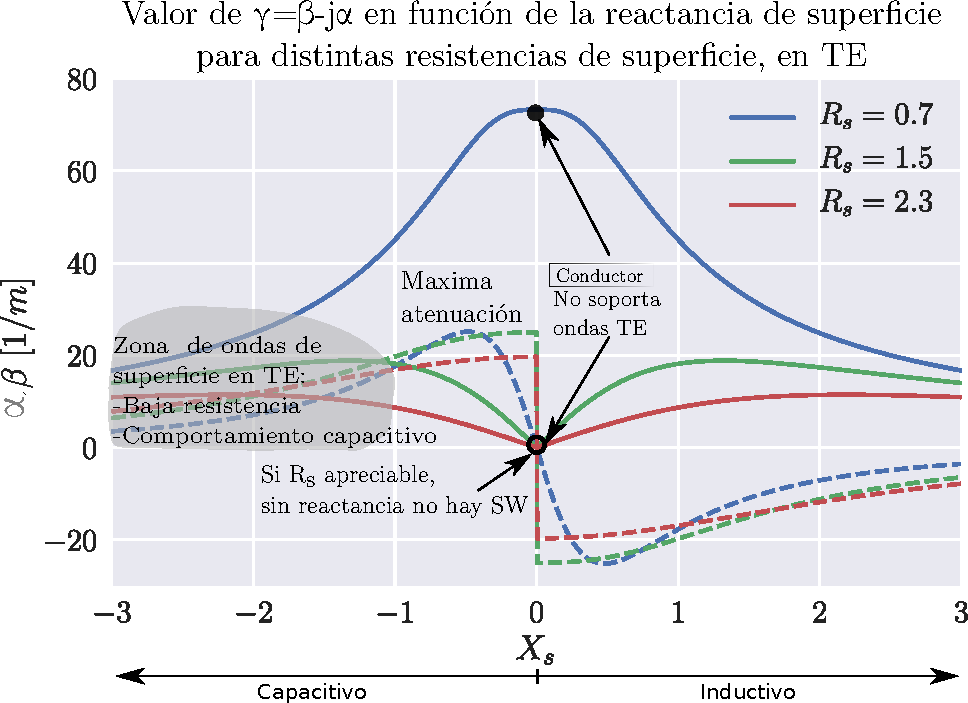
\includegraphics[width=\textwidth]{intro_electro/plot-beta-reactancia-TE.pdf}
	%\input{Figures/intro_electro/onda-superficie-incidencia-brewster3.pdf_tex}
	\caption{Comportamiento de la constante de propagación superficial $\beta$ en función de la resistencia y reactancia superficial para el caso de incidencia TE. Las líneas punteadas representan la parte imaginaria de $\beta$, y las líneas completas representan la parte real, de forma que $\beta = \beta' - j\beta''$.}
	\label{fig:beta-reactancia-TE}
\end{figure}

Entre las distintas formas de lograr que una interfaz conductor-aire permita el guiado de ondas de superficie, una de las más efectivas consiste en el recubrimiento de la superficie metálica por una capa dieléctrica fina, como se muestra en la figura \ref{fig:thin-dielectric-coating}.

\begin{figure}[htp]
	\centering
	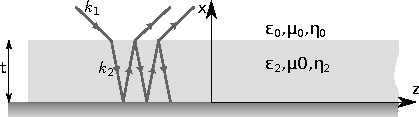
\includegraphics[width=0.7\textwidth]{intro_electro/incidencia-coated-conductor.pdf}
	\caption{Incidencia sobre un conductor recubierto por un dieléctrico.}
	\label{fig:thin-dielectric-coating}
\end{figure}

Para el caso TM, si se considera que el campo magnético tiene la forma de la ecuación \ref{eq:campo-magnetico-TM} en el espacio libre circundante a la estructura, entonces el campo magnético en el interior del dieléctrico resultará de la forma expresada en la ecuación \ref{eq:campo-magnetico-interior-diel-TM}, donde se cumple que $h_1^2 + \beta^2 = k_0^2$ y $h_2^2 + \beta^2 = k^2 = \epsilon_r k_0^2$.

\begin{align}
	\label{eq:campo-magnetico-TM}
	H_{1_y} = A e^{jh_1x - j \beta z},\quad x>t
\end{align}

\begin{align}
	\label{eq:campo-magnetico-interior-diel-TM}
	H_{2_y} = [B e^{jh_2 x} + C e^{-jh_2 x}] e^{-j\beta z},\quad  0\leq x \leq t
\end{align}

Dado que en toda interfaz las componentes tangenciales de los campos se conservan, y a que las componentes tangenciales del campo eléctrico sobre el conductor se anulan, se deduce que $H_{2_y}$ es un coseno, y se obtienen\footnote{De la ecuación \ref{eq:campo-magnetico-TM} se deriva el campo eléctrico, utilizando la ecuación de Ampère. Al establecer la condición que indica que sobre la interfaz con el conductor no existe campo eléctrico paralelo a la superficie del mismo (se asume un conductor perfecto), se concluye que el valor de B y de C en la ecuación \ref{eq:campo-magnetico-interior-diel-TM} coinciden. Aplicando la condición de continuidad de las componentes tangenciales de los campos sobre la interfaz aire-dieléctrico, se obtiene una relación entre los valores de A y B. Queda expresado el siguiente sistema de ecuaciones:
\begin{equation*}
	\begin{bmatrix}
		-j h_1 e^{-j h_1 t} & -2 h_2/\epsilon_{r_2} \sin(h_2 t) &  \\
		 -e^{-j h_1 t} & 2 \cos (h_2 t)
	\end{bmatrix}
	\begin{bmatrix}
		A \\
		B
	\end{bmatrix}
	=
	\begin{bmatrix}
		0 \\
		0
	\end{bmatrix}
\end{equation*}

Para que la solución no sea trivial, el determinante de la matriz del sistema tiene que ser nula, lo que da como resultado $h_2 \tan (h_2 t) = -j h_1 \epsilon_{r_2}$.
} las expresiones \ref{eq:solucion-ondas-sup-tm-tan} y \ref{eq:solucion-ondas-sup-tm-h}.


\begin{align}
	\label{eq:solucion-ondas-sup-tm-tan}
	h_2 \tan (h_2 t) = -j h_1 \epsilon_{r_2} \\
	k_0^2 (\epsilon_{r_2}-1) = h_2^2 - h_1^2
	\label{eq:solucion-ondas-sup-tm-h}
\end{align}

Considerando que $h_1$ es puramente complejo positivo\footnote{Un análisis general requiere considerar $h_1$, $h_2$ y $\epsilon_2$ como complejos, de manera que se puedan considerar las pérdidas. Para simplificar el desarrollo, se debe considerar que, dado que se trata de ondas de superficie, la parte imaginaria de $h_1$ deberá ser negativa, de manera que a mayor distancia de la interfaz, la intensidad de los campos decrezca exponencialmente. La parte real de $h_1$, si bien puede existir, a efectos del estudio del comportamiento de la onda de superficie en la dirección de propagación, puede obviarse. Por otro lado, si se considera que el ancho del dieléctrico, $t$, es muy pequeño, de forma que se pueda considerar que $\tan(h_2 t) \approx h_2 t$, entonces la expresión \ref{eq:solucion-ondas-sup-tm-tan} resulta aproximadamente $h_2^2 t = -j h_1 \epsilon_{r_2}$. Asumiendo, por lo explicado antes, que $h_1$ es valor puramente imaginario positivo, el valor de $h_2$, obtenido de $h_2^2 t = h_1 \epsilon_{r_2}$, deberá ser real. Al argumento no descarta la existencia de valores complejos de $h_1$ y $h_2$, sino que permite una validación intuitiva del desarrollo posterior.}, la ecuación \ref{eq:solucion-ondas-sup-tm-h} se puede expresar como $k_0^2 (\epsilon_{r_2}-1) = h_2^2 + |h_1|^2$. Si se multiplica esta nueva expresión por $t^2$ y a la expresión \ref{eq:solucion-ondas-sup-tm-tan} por $t$, se obtienen dos expresiones que dan lugar a un sistema de ecuaciones trascendentales que se pueden resolver gráficamente, dado que representan una esfera de radio $k_0 t \sqrt{\epsilon_{r_2}-1}$ y una tangente:

\begin{equation}
	\label{eq:sistema-ondas-superficiales-TM}
	\begin{cases}
		(h_2 t)^2 + (h_1 t)^2 = (\epsilon_{r_2} - 1) (k_0 t)^2\\
		h_2 t \tan (h_2 t) = |h_1| \epsilon_{r_2} t
	\end{cases}
\end{equation}

Para el caso TE, la solución es similar, y en este caso las expresiones resultan (considerando, nuevamente, que $h_1$ es puramente imaginario positivo):

\begin{equation}
	\label{eq:sistema-ondas-superficiales-TE}
	\begin{cases}
		(h_2 t)^2 + (h_1 t)^2 = (\epsilon_{r_2} - 1) (k_0 t)^2 \\
		h_2 t \cot (h_2 t) = -|h_1| \epsilon_{r_2} t
	\end{cases}
\end{equation}

Las soluciones se pueden obtener gráficamente para ambos casos, mediante la intersección de las curvas correspondientes a las ecuaciones del sistema. Las gráficas, para distintas frecuencias, se muestran en la figura \ref{fig:intersecciones-tm-te}. Se puede observar que, dado que $|h_1|t$ no puede tomar valores negativos, las intersecciones que se dan en esas condiciones no son válidas como soluciones del sistema planteado, bajo las hipótesis consideradas.

A medida que aumenta la frecuencia, el valor del radio de los círculos aumenta. Se observa que siempre existe, al menos, un modo TM de propagación sobre el plano de tierra, dado que todas las intersecciones entre las curvas ocurren para valores de $|h_1| t$ mayores a 0, como se muestra en la figura \ref{fig:soluciones-TM-tan-implicita-zoom}. Para frecuencias en que el radio del círculo genera que el mismo intersecte a más secciones de la curva tangente, aparecerían modos de propagación superiores.

Para el caso TE, se observa que para frecuencias bajas no existe solución válida, como se muestra en la figura \ref{fig:soluciones-TE-tan-implicita-zoom}, por lo que no hay un modo fundamental TE por debajo de la frecuencia de corte, que se da para $f_c = c/(4 t  \sqrt{\epsilon_{r_2}}-1)$, que en el caso graficado es de aproximadamente 25 GHz.

Para el caso de FR4, en el rango de frecuencias de interés para este trabajo, no existe, entonces, propagación de ondas de superficie de polarización TE, por lo que el análisis del modo TM reviste mayor importancia.


\begin{figure} [H]
	\centering 
	\subfigure[TM]{
		\label{fig:soluciones-TM-tan-implicita}
		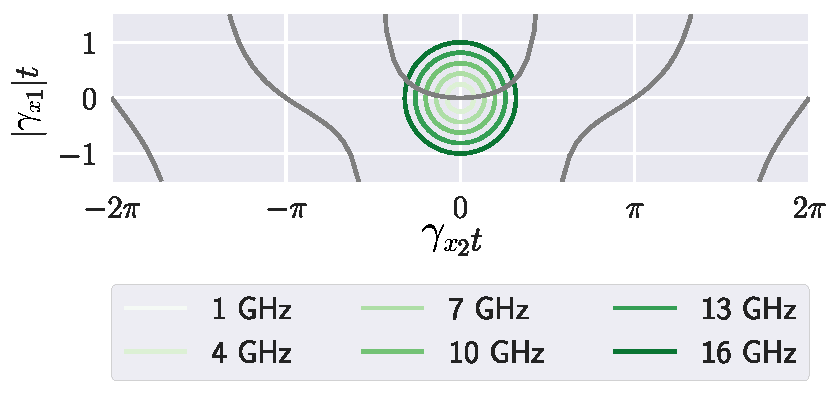
\includegraphics[width=0.48\textwidth]{intro_electro/TM-tan-implicito}}
	\subfigure[TE]{
		\label{fig:soluciones-TE-tan-implicita}
		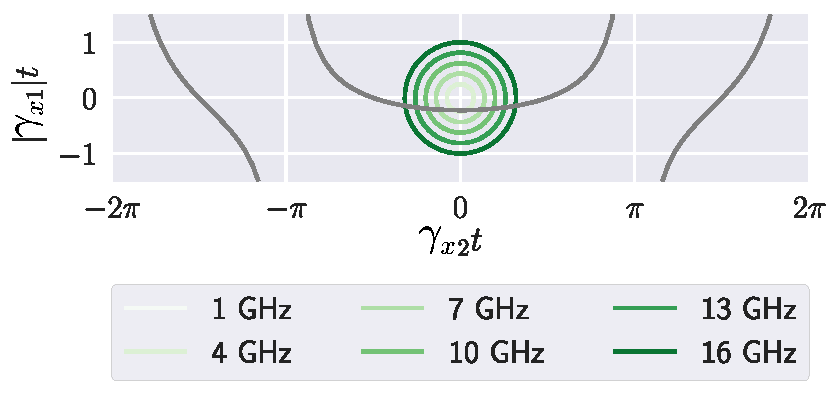
\includegraphics[width=0.48\textwidth]{intro_electro/TE-tan-implicito}}
	\subfigure[Zoom para modo TM]{
		\label{fig:soluciones-TM-tan-implicita-zoom}
		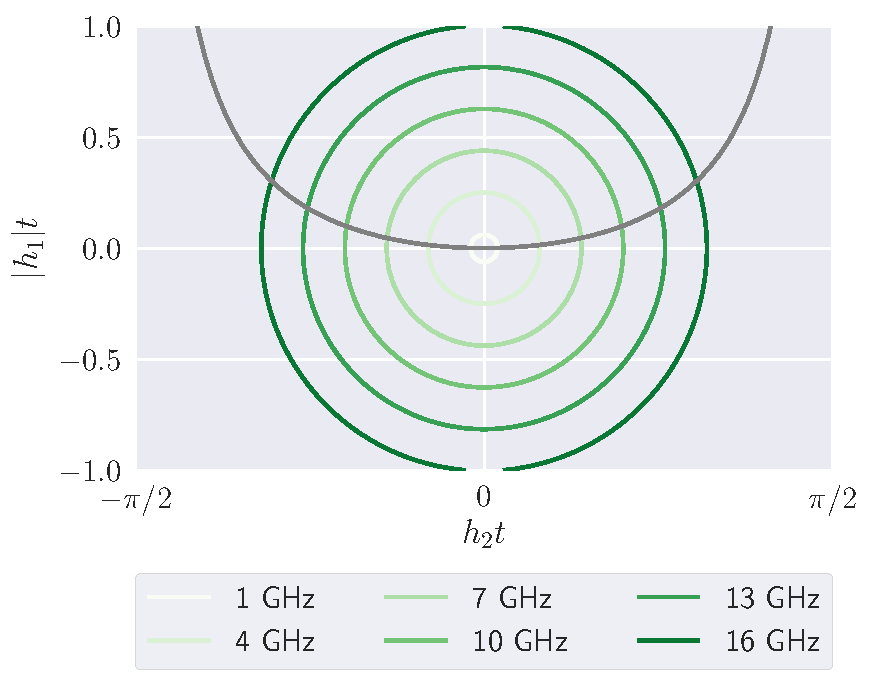
\includegraphics[width=0.48\textwidth]{intro_electro/TM-tan-implicito-zoom}}
	\subfigure[Zoom para modo TE]{
		\label{fig:soluciones-TE-tan-implicita-zoom}
		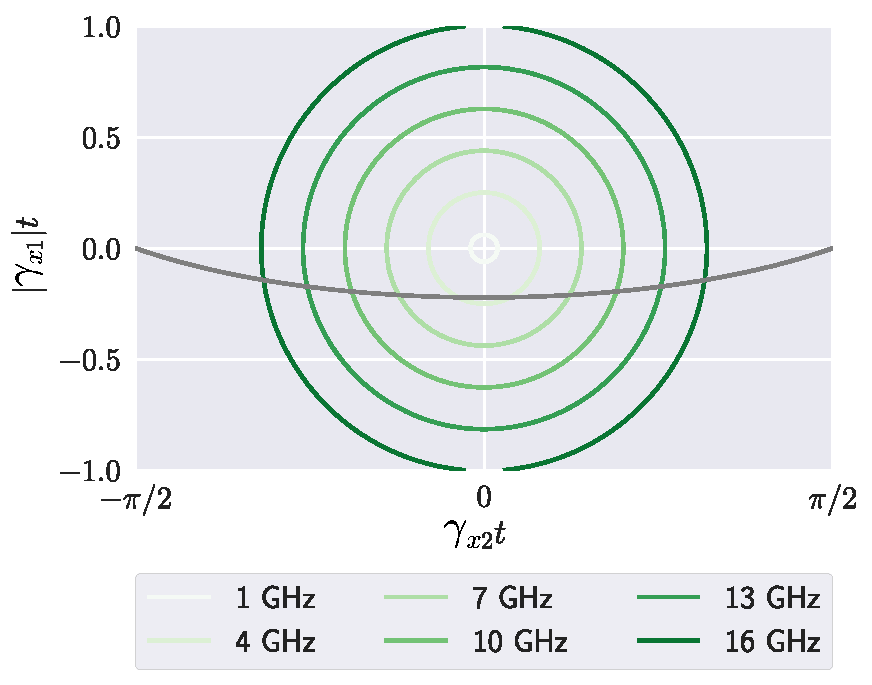
\includegraphics[width=0.48\textwidth]{intro_electro/TE-tan-implicito-zoom}}
	\caption{Curvas de los sistemas de ecuaciones que describen la existencia de ondas superficiales TM y TE, para distintas frecuencias, resuelto para el caso en que el dieléctrico es FR4 ($\epsilon_r = 4.5$).}
	\label{fig:intersecciones-tm-te}
\end{figure}

Obtenidos los valores de $h_1$ y $h_2$, se obtienen los campos del modo correspondiente de la onda de superficie \cite{Pozar:MwEngineering}. En particular, para el análisis del comportamiento de la impedancia, las expresiones de los campos tangenciales a la interfaz resultan de mayor interés, dado que permiten obtener las impedancias de onda en el aire y el dieléctrico, como se indica en las expresiones \ref{eq:impedancia-no-normalizada-aire} y \ref{eq:impedancia-no-normalizada-FR4}.

\begin{subequations}
	\begin{align}
		H_{y_1} &= A e^{jh_1(x-t)-j\beta z}, &E_{z_1} &= \frac{A h_1}{\omega \epsilon_0} e^{jh_1(x-t)-j\beta z} &\implies& Z_1 = \frac{h_1}{\omega \epsilon_0} \label{eq:impedancia-no-normalizada-aire}\\
		H_{y_2} &= 2 B \cos(h_2 x) e^{j\beta z}, &E_{z_2} &=  \frac{-2 B h_2 \sin(h_2 x)e^{-j\beta z}}{j \omega \epsilon_0 \epsilon_{r_2}} &\implies& Z_2 = \frac{jh_2 \tan(h_2 x)}{\omega \epsilon_0 \epsilon_{r_2}} \label{eq:impedancia-no-normalizada-FR4}
	\end{align}
\end{subequations}

Normalizando respecto de la impedancia intrínseca del vacío, $\eta_0$, se obtiene, considerando $\theta_t$ el ángulo de transmisión desde el aire al dieléctrico que recubre el plano conductor,:

\begin{align}
	\frac{Z_{1}}{\eta_0} &= \frac{h_1}{\omega \epsilon_0 \eta_0} = \frac{k_0 \cos\theta_i}{\omega \epsilon_0 \eta_0} = \cos \theta_i \\
	\frac{Z_{2}}{\eta_0} &= j\frac{h_2 \tan h_2 x}{\omega \epsilon_0 \epsilon_{r_2} \eta_0} = j\frac{k_2 \cos\theta_t \tan(k_2 x \cos\theta_t)}{\omega \epsilon_0 \epsilon_{r_2} \eta_0} = j \frac{\cos \theta_t}{\sqrt{\epsilon_{r_2}}}\tan(k_2 x \cos\theta_t)
\end{align}

Una onda incidente desde el aire, para evitar reflexiones y, por lo tanto, radiación desde la superficie que soporta una onda de superficie, debe estar adaptada a la impedancia de superficie que presenta el dieléctrico, que resulta de evaluar $Z_2/\eta_0$ en la superficie:

\begin{align}
	Z_s = j \frac{\cos \theta_t}{\sqrt{\epsilon_{r_2}}}\tan(k_2 t \cos\theta_t)
\end{align}

%% GRAFICAR!!! \theta_r puede ser obtenida por la ley de snell. Vemos que no es independiente del ángulo de incidencia. Barlow dice que son del mismo orden de magnitud los efectos viejos (prof de penetracion) y los nuevos (coating). Pagina 332. Carita triste.

% Barlow parece contar cosas sobr la velocidad de fase, y más dealnte sobre el lauching y el angulo de brewster complejo. LEER para completar.

Esta impedancia es puramente imaginaria positiva\footnote{Si el dieléctrico presentara pérdidas, existiría también un término real \cite{Barlow:SurfaceWaves}, por lo que, además de facilitar la propagación de ondas de superficie, si el dieléctrico tiene bajas pérdidas, no aumenta la resistencia de superficie. Además, esta componente inductiva se debe sumar al efecto producido por la componente inductiva de la impedancia de superficie del conductor, debida a la existencia de una profundidad de penetración.}, por lo que tiene un comportamiento inductivo, permitiendo la formación de ondas de superficie en modo TM, dado que la constante de atenuación $h''$ logra que el campo se concentre cerca de la superficie. Los valores de $\beta'$ y $\beta''$ no se ven modificados, pues el aporte del dieléctrico a la reactancia no es lo suficientemente alto. El ángulo $\theta_t$ se obtiene de las relaciones de Snell (\ref{eq:snell_law_second}), por lo que se deduce que, al contrario que en el caso del conductor sin recubrimiento dieléctrico, el comportamiento es dependiente del ángulo de incidencia.

% Queda explicar qué pasa con el coating -> ubicar también los puntos en el dibujito, para saber por dónde es que nos movimos.


% Engheta, pagina 289
% Rahim (tesis), pagina 28
% Collin, capitulo de Surface waveguides, pag 697
% Paper de Barlow.
% Pozar, pag 138
% Tesis de Kovacs, pagina 8
% Tesis de Zheng, apendice A, pag 48. Interfaces con diel y con metales.


\section{Líneas de transmisión}
\label{sec_lineas_de_transmision}
%%%%

%  Cuando los metamateriales son homogéneos, pueden ser representados por líneas de transmisión unidimensionales, donde la dirección representa cualquier dirección en el material (Caloz, Itoh).

La teoría de líneas de transmisión representa el paso intermedio entre el estudio de campos electromagnéticos y de circuitos impresos, permitiendo considerar el fenómeno de propagación de ondas como una extensión de la teoría de circuitos (aplicable cuando la longitud eléctrica del circuito es mayor a la longitud de onda de operación), o como una solución particular de las ecuaciones de Maxwell \cite{Pozar:MwEngineering}.

Las líneas de transmisión son redes de parámetros distribuidos, donde las corrientes y las tensiones, en contraposición a los circuitos de parámetros concentrados, pueden variar en magnitud y fase debido a la dimensión física del circuito. El análisis de una línea se puede llevar a cabo estableciendo el comportamiento de los trozos infinitesimales que la componen, de forma que cada uno de ellos se pueda modelar utilizando circuitos de parámetros concentrados independientes de la frecuencia, estableciendo, entonces, impedancias $Z'$ ($\Omega/m$) y admitancias $Y'$ ($S/m$) por unidad de longitud, como se muestra, de forma general, en la figura \ref{fig:TL-equivalente}.

\begin{figure}[htp]
	\centering
	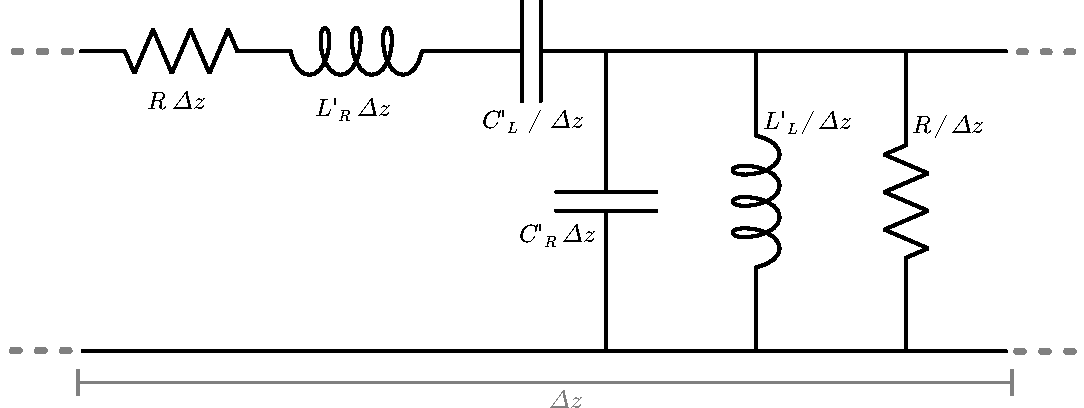
\includegraphics[width=0.8\textwidth]{intro_electro/LineaDeTransmision.pdf}
	\caption{Circuito equivalente de porción de línea de transmisión.}
	\label{fig:TL-equivalente}
\end{figure}

Las expresiones para la impedancia y la admitancia por unidad de longitud se puede expresar como indican las expresiones de \ref{eq:impedancia-admitancia-TL}. Se debe tener en cuenta que los subíndices R y L se deben al comportamiento de "mano izquierda"\footnote{La expresión "material de mano izquierda" fue utilizada por primera vez por físico ruso Viktor Velesago en 1967, cuando propuso la posibilidad de la existencia de materiales en que la propagación de ondas se daría de forma que el campo eléctrico, el campo magnético y el vector de propagación formaran una tríada de mano izquierda \cite{Caloz}.} o ``mano derecha`` asociado a cada componente. Si $L'_R$ y $C'_R$ son nulos, existe sólo un comportamiento "de mano izquierda", donde las velocidades de fase y de grupo son antiparalelas, y donde tanto la permitividad eléctrica $\epsilon$ como la permeabilidad magnética $\mu$ son negativas, de forma que el índice de refracción también lo sea, dando lugar a una propagación de ondas en sentido inverso. Cuando $L'_L$ y $C'_L$ son nulos, el comportamiento es denominado "de mano derecha", y es el que corresponde a propagación de onda comunmente analizada. Las componentes que corresponden al comportamiento de mano izquierda son, por sí solas, de existencia física imposibles, dado que las que generan comportamiento de mano derecha aparecen naturalmente por efectos constructivos. Las resistencias del circuito, por otro lado, representan las pérdidas dieléctricas y conductoras.


\begin{align}
\label{eq:impedancia-admitancia-TL}
Z' &= j \left(\omega L'_r - \frac{1}{\omega C'_L} \right) & Y' =j \left(\omega C'_R - \frac{1}{\omega L'_L} \right)
\end{align}

Una descripción completa del análisis del caso general, que describe el comportamiento de numerosos metamateriales, se puede consultar en \cite{Caloz}. En adelante se analizará únicamente el caso tradicional, de mano derecha, ya que es el que se aplica al tipo de estructura analizado en este trabajo.

Considerando una línea de transmisión que representa un comportamiento puramente de mano derecha, obteniendo el circuito equivalente de un infinitesimal de línea de la figura \ref{fig:TL-equivalente}, aplicando las leyes de Kirchhoff, y dividiendo por $\Delta z$ para obtener expresiones diferenciales, se obtienen las ecuaciones del telegrafista, expresadas en la ecuación \ref{eq:Telegrafista}, tanto en el dominio del tiempo como de la frecuencia \cite{Fernandez:Electromag}. La solución simultánea de ambas ecuaciones da lugar a ecuaciones de onda, expresadas en \ref{eq:ec-onda-TL}, donde $\gamma$ es la constante de propagación, cuyo valor se expresa \ref{eq:gamma-tl}.

\begin{align}
	\label{eq:Telegrafista}
	\left. \begin{array}{rr@{\mskip\thickmuskip}l}
	\frac{\partial v(z,t)}{\partial z} & = -R i(z,t) - L \frac{\partial i(z,t)}{\partial t}\\
	\frac{\partial i(z,t)}{\partial z} & = -G v(z,t) - C \frac{\partial v(z,t)}{\partial t}
	\end{array}\right\} \quad \implies \quad \left\{\begin{array}{r@{\mskip\thickmuskip}l}
	\frac{dV(z)}{dz} & = -(R+j\omega L)I(z) \\
	\frac{dI(z)}{dz} & = -(G+j\omega C)V(z) 
	\end{array}\right.
\end{align}


\begin{equation}
\begin{aligned}
	\frac{d^2 V(z)}{dz^2} - \gamma^2 V(z) = 0 \\
	\frac{d^2 I(z)}{dz^2} - \gamma^2 I(z) = 0
\end{aligned}
\label{eq:ec-onda-TL}
\end{equation}

\begin{align}
	\label{eq:gamma-tl}
	\gamma = \alpha + j\beta = \sqrt{(R+j\omega L)(G+j\omega C)}	
\end{align}

 Las ecuaciones de onda tienen como solución la superposición de una onda en dirección $+z$ y otra en dirección $-z$, tanto para la tensión como para la corriente, donde la longitud de onda queda expresada como $\lambda = \pi/\beta$. La relación entre las componentes de onda que viajan en dirección positiva se conoce como impedancia característica, $Z_0$, definida, según los parámetros, en la ecuación \ref{eq:TL-impedancia-caracteristica}.
 
\begin{align}
	\label{eq:TL-impedancia-caracteristica}
	Z_0 = \frac{V_0^+}{I_0^+} = \sqrt{\frac{R+j\omega L}{G+j\omega C}}
\end{align}

Cuando una línea de transmisión es terminada en una impedancia arbitraria $Z_L$, se producen fenónemos de transmisión y reflexión de potencia, de manera análoga al caso de incidencia de campos electromagnéticos sobre interfaces entre medios de impedancias intrínsecas diferentes. Existe, también en este caso, un coeficiente de reflexión $R$, definido como la relación entre la tensión reflejada y la tensión incidente, como indica la ecuación \ref{eq:coef-reflexion-tl}. Cuando el coeficiente de transmisión es nulo, se dice que la carga está adaptada, de modo que $Z_L = Z_0$.

\begin{align}
	\label{eq:coef-reflexion-tl}
	R = \frac{V_0^-}{V_0^+} = \frac{Z_L-Z_0}{Z_L+Z_0}
\end{align}

Si se generaliza el concepto de coeficiente de transmisión a cualquier punto de la línea, y no únicamente al nodo donde se coloca la carga $Z_L$, se obtiene el coeficiente de reflexión para cualquier punto $l$ de la línea a partir del que corresponde al nodo de carga, ubicado en la posición 0, como se indica en la ecuación \ref{eq:coef-reflexion-tl-generalizado}.

\begin{align}
\label{eq:coef-reflexion-tl-generalizado}
R(l) = Re^{-2j\gamma l} = R e^{-2j\beta l} e^{-2\alpha l}
\end{align}

La impedancia característica también varía con la distancia a la carga, de forma que:

\begin{align}
Z_{in} = \frac{V(-l)}{I(-l)} = Z_0 \frac{Z_L +Z_0 \tanh \gamma l}{Z_0 + Z_L \tanh \gamma l}
\end{align}
% Venkateswaran, cap 1.
%%%%
\subsection{Línea \textit{microstrip}}

Algunas de las líneas de transmisión más comunes están basadas en tecnologías de circuitos impresos, entre las que se destacan las striplines (donde el dieléctrico circundante al conductor es homogéneo), las líneas \textit{microstrip} (donde el dieléctrico circundante es aire en la mitad superior, y un dieléctrico de mayor permitividad en la mitad inferior), y las guías de ondas coplanares (donde el plano de tierra y la línea de señal comparten la misma cara del sustrato). Algunas de ellas son esquematizadas en la figura \ref{fig:strip-line-technology}. Los costos de fabricación de las mismas suelen ser muy bajos, y ofrecen comodidades para la implantación de componentes discretos, aunque en muchos casos se generan modos indeseados, que pueden ser disminuidos manteniendo el espesor del sustrato en valores bajos, lo que los vuelve frágiles. Además, los sustratos dieléctricos suelen presentar pérdidas que modifican el comportamiento de la señal. Las principales aplicaciones consisten en el diseño de filtros microondas, acopladores direccionales, transformadores de impedancia, planos de tierra y redes de distribución de energía de circuitos impresos e integrados \cite{Venkateswaran}.


\begin{figure}[htp]
	\centering
	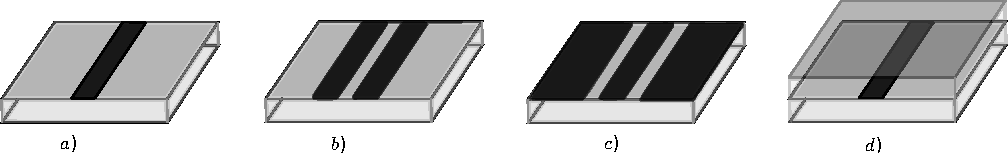
\includegraphics[width=\textwidth]{intro_electro/microstrip-stripline-coplanar.pdf}
	\caption{Tecnologías de líneas de transmisión planares. De izquierda a derecha: \textit{Microstrip}, \textit{twinstrip}, línea coplanar y \textit{stripline}.}
	\label{fig:strip-line-technology}
\end{figure}

Las striplines, debido a la homogeneidad del dieléctrico, soportan modos TEM. Las líneas microstrip, en cambio, sólo pueden presentar modos TE y TM, aunque en frecuencias bajas tienen un comportamiento que puede denominarse cuasi-TEM, dado que la mayor parte del campo se concentra en el dieléctrico, pero un comportamiento puramente TEM impediría el cumplimiento de la condición de fase en la interfaz, dado que las velocidades de propagación en ambos medios es distinta \cite{Pozar:MwEngineering}. Un diagrama simplificado de los campos y los parámetros de una línea microstrip se muestran en la figura \ref{fig:microstrip-campos}


\begin{figure}[htp]
	\centering
	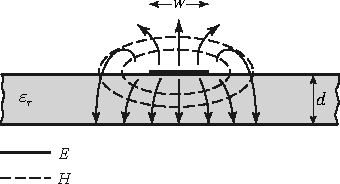
\includegraphics[width=0.5\textwidth]{intro_electro/microstrip-campos.pdf}
	\caption{Campos de una línea \textit{microstrip}.}
	\label{fig:strip-line-technology}
\end{figure}

En general, para simplificar el análisis, se considera que la cinta microstrip es una stripline, donde el dieléctrico tiene una constante dieléctrica efectiva, menor a la constante dieléctrica del sustrato, pero mayor a la del aire, dependiente del ancho del sustrato, el ancho del conductor y la frecuencia de trabajo. Las expresiones pueden consultarse en \cite{Pozar:MwEngineering}.

\section{Antenas}
\label{subsec_antenas}
%%%%

Una antena es un dispositivo que actúa como fuente de ondas electromagnéticas, dado que es una interfaz entre el espacio libre y un dispositivo de guiado (como una guía de ondas), para la cual puede ser modelada como una carga (en general, adaptada). Su función es recibir o transmitir energía, usualmente optimizando la energía en algunas direcciones, y suprimiendo o disminuyendo su valor en otras, para lo que se utilizan distintas tecnologías: antenas de hilo, de apertura y microstrip, muchas veces dispuestas en arreglos y con componentes reflectores \cite{Balanis:Theory}.

%%%%
\subsection{Regiones de campo}
\label{subsubsec_regiones_de_campo}
%%%%
El espacio que rodea a una antena se suele dividir en tres regiones: Campo cercano reactivo (donde predominan los campos reactivos), campo de radiación cercano (Fresnel, donde la distribución angular de energía depende de la distancia a la antena) y campo lejano (Fraunhoffer, donde la distribución angular de energía es, en términos prácticos, independiente de la distancia al elemento radiante). En general, se considera que la región de campo lejano se encuenta a distancias mayores a $2D^2/\lambda$, donde D es la máxima dimensión de la antena, y $\lambda$ es la longitud de onda de trabajo.

%%%%
\subsection{Diagramas de radiación}
\label{subsubsec_diag_de_rad}
%%%%
El diagrama de radiación es una representación gráfica o función matemática que representa las propiedades de radiación de una antena como función d elas coordenadas espaciales. En general, se especifica para la región de campo lejano, y en función de las coordenadas direccionales $\theta$ y $\phi$, que representan el ángulo de elevación y el azimutal, respectivamente, para una orientación arbitraria del radiador.

En general, se calcula el patrón de potencial o el patrón de campo eléctrico, y se los normaliza respecto del máximo valor que obtienen, para luego graficarlos en escala logarítima o en decibeles.

Sobre el patrón se distinguen lóbulos, clasificados como principal (en la dirección de mayor radiación) y menores (en otras direcciones). Si una antena es isotrópica, esta distinción no existe, aunque es físicamente irrealizable. Cuando no existen lóbulos distinguibles en un dado plano, la antena se clasifica como omnidireccional.
%%%%

\subsection{Impedancia de entrada}
\label{subsec_imp_entrada}
%%%%
La impedancia de entrada de una antena es la que presenta una antena entre sus terminales. En general tiene una componente resistiva y una componente reactiva, de manera que $Z_A = R_A + j X_A$. En general, $R_A$ tiene dos componentes: $R_r$, la resistencia de radiación, y $R_L$, la resistencia de pérdidas.
%%%%

\subsection{Arreglos de antenas}
% Ver apunte tesis overleaf

\subsection{Acoplamiento mutuo}
\label{subsec_acoplamiento}
%%%%
\lipsum[2]
%Paper de fano y el cordobeés.
%%%%
\subsection{Dieléctricos y pérdidas dieléctricas}
\label{subsec_dielectricos}
%%%%
\lipsum[2]
% LibroSinNombre, pagina 816
%%%%
\subsection{Parámetros S}
\label{subsec_parametros_s}
%%%%
\lipsum
% Pozar, pag 178
%%%%

\subsection{Antenas Microstrip}
\label{subsec_antenas_microstrip}
%%%%
\lipsum
%%%%
\subsubsection{Modelo de líneas de transmisión}
\label{subsubsec_microstrip_modeloLineas}
%%%%
\lipsum
% LibroSinNombre, pahgina 534
%%%%
\subsubsection{Modelo de cavidades multimodo}
\label{subsubsec_microstrip_modeloCavidades}
%%%%
\lipsum

% Pozar, rezonadores, capitulo 6
%%%%

\subsection{Acoplamiento mutuo en antenas Microstrip}
\label{subsec_acoplamiento_microstrip}
%%%%
\lipsum
%%%%
% LibroSinNombre, pagina 562 y 631


